\documentclass[12pt]{article}

\usepackage[T1]{fontenc}
\usepackage[utf8]{inputenc}
\usepackage{mathptmx}
\usepackage{microtype}
\usepackage[margin=1in]{geometry}
\usepackage{setspace}
\usepackage{amsmath}
\usepackage{graphicx}
\usepackage{booktabs}
\usepackage{longtable}
\usepackage{tikz}
\usetikzlibrary{arrows.meta}
\usepackage{titletoc}
\usepackage[authordate,backend=biber,natbib=true,noibid]{biblatex-chicago}
\addbibresource{references.bib}
\usepackage{hyperref}
\hypersetup{colorlinks=true, linkcolor=black, citecolor=black, urlcolor=black}
\usepackage{xurl}
\setcounter{tocdepth}{2}
\graphicspath{{fig/}{../docs/fig/}{../csv_exports/}}

\title{\textbf{AI-Driven High School Data Intelligence Platform}}
\date{Summer 2026}

\begin{document}

% ---------------------------------------------------------------------
% TITLE PAGE
% ---------------------------------------------------------------------
\begin{titlepage}
\centering
\vspace*{3cm}

{\LARGE \textbf{AI-Driven High School Data Intelligence Platform}}\\[0.6cm]
{\Large Linking, Classifying, and Auditing U.S. High Schools for College Admissions Context}\\[2.5cm]

{\large Max Chalekson}\\
{\large Sheng Hu}\\
{\large Qifan Yang}\\[1.5cm]

Northwestern University\\
Master of Science in Data Science\\[1.5cm]

Prepared for Bob Henkins\\
Northwestern Undergraduate Admissions and Enrollment\\[3cm]

\vfill
Summer 2026

\end{titlepage}

\pagenumbering{roman}

% ---------------------------------------------------------------------
% ABSTRACT
% ---------------------------------------------------------------------
\section*{Abstract}
\addcontentsline{toc}{section}{Abstract}
\noindent College admissions offices lack standardized information about the high schools their applicants attend, and the College Board discontinued Landscape, the closest thing to a common answer, in September 2025. This paper reports the design, construction, and evaluation of a replacement built for one institution: an internally owned, publicly sourced, auditable platform that links, classifies, and contextualizes United States high schools. Sixteen public data sources plus the client's own organization export were consolidated into a Dockerized PostgreSQL database and two frozen analytical datasets covering 34{,}392 high schools and 45{,}250 client organization records. Schools were linked across NCES, CEEB, and OPE identifier systems using a Fellegi--Sunter accept/review/reject decision rule, with rules resolving 88 percent of ambiguous pairs and a large language model adjudicating the remainder. A nine-component weighted rigor index was cut into five ordinal tiers by Jenks natural breaks. Three results are central. First, measured effective weights diverge sharply from designed weights: Advanced Placement exam performance contributes 0.364 of index variance against a nominal 0.20, confirming that performance, not course availability, carries the signal. Second, the index reproduces socioeconomic ordering measurably ($\rho = -0.32$ with child poverty), so a second, orthogonal opportunity-adjusted measure was added; it surfaces five times as many high-need overperforming schools as the raw tier. Third, opportunity structure predicts graduation beyond socioeconomic status by only 0.04--0.05 in $R^2$. Clustering was weak by design standards and is reported as a finding about the data.
\bigskip

\noindent\textbf{Keywords:} record linkage, composite indicators, college admissions, school context, reproducible pipelines

\bigskip
\noindent\textbf{Data and code availability.} The public sources are cited in Section~\ref{sec:data} and listed with vintages in Appendix~\ref{app:sources}. The compiled database and its derived assignments were developed for the client and are not publicly released; the pipeline rebuilds through \texttt{docker compose up -{}-build} in a repository private to the capstone team and the client.

\medskip
\noindent\textbf{Acknowledgements.} The authors thank Bob Henkins and Northwestern Undergraduate Admissions and Enrollment for sponsoring this project, and the Northwestern University Master of Science in Data Science program for its support.

\newpage
\tableofcontents
\newpage

\pagenumbering{arabic}
\setcounter{page}{1}
\doublespacing

% ---------------------------------------------------------------------
% INTRODUCTION
% ---------------------------------------------------------------------
\section{Introduction}
\label{sec:introduction}

A student's transcript arrives at an admissions office without the context needed to interpret it: how many Advanced Placement (AP) or International Baccalaureate (IB) courses the school offers, how its per-student funding compares to peers, or where its average SAT sits relative to similar schools. \citet{bastedo2023} find that admissions officers lack high school context on roughly a quarter of applications, with public and majority-low-income schools least likely to supply it. For a decade the College Board's Environmental Context Dashboard and its successor, Landscape, were the closest thing to a standardized answer. Neither exists as of September 2025, and, as Section~\ref{sec:prior-art} shows, the withdrawal had nothing to do with whether the tool worked.

\textbf{Problem statement.} No available tool gives admissions offices school context that is simultaneously honest about measuring curricular \emph{opportunity} rather than student \emph{outcome}, decomposable to the data behind every score, checked against reproducing the socioeconomic ordering of American schools, and owned by the institution that depends on it rather than licensed from a vendor who can withdraw it. Landscape came closest and is gone.

Northwestern University's Undergraduate Admissions and Enrollment office, represented by Bob Henkins, commissioned this capstone to build that platform. The delivered system consolidates sixteen public data sources and the client's own organization export into a Dockerized PostgreSQL database, links schools across the NCES, CEEB, and OPE identifier systems, scores each school on a nine-component curricular rigor index cut into five ordinal tiers, emits a second opportunity-adjusted score built for gap detection, clusters schools and colleges, and benchmarks test performance against peer groups. Every number below is reproducible from frozen, dated artifacts in the project repository. Section~\ref{sec:literature-review} reviews the four literatures bearing on the design and states the gap; Section~\ref{sec:data} describes the data and linkage; Section~\ref{sec:methods} the methodology; Section~\ref{sec:results} the results; and Sections~\ref{sec:discussion}--\ref{sec:future-work} interpret them.

% ---------------------------------------------------------------------
% LITERATURE REVIEW
% ---------------------------------------------------------------------
\section{Literature Review}
\label{sec:literature-review}

\subsection{Three findings that revised the project plan}

Three findings contradicted or qualified the project's own plan and changed what was built.

First, the plan asserted that no public source publishes school-level AP participation. That is incorrect. The Civil Rights Data Collection (CRDC), a biennial census of public schools receiving federal funds, publishes school-level AP course counts and enrollment, IB enrollment, dual enrollment, SAT/ACT participation, and advanced mathematics and science offerings, keyed to NCES identifiers with no fuzzy matching required \citep{ocr_crdc}. It does not publish AP exam \emph{scores}, so the coursework-versus-performance distinction below still binds, but it removed a hard dependency on a College Board institutional-access request that never arrived.

Second, the College Board discontinued Landscape in September 2025 for post-\textit{SFFA v. Harvard} legal and political reasons rather than commercial ones (Section~\ref{sec:prior-art}), which makes the plan's assertion that no governmental or socio-cultural considerations apply difficult to sustain.

Third, the federal infrastructure both findings rely on is fragile. The National Center for Education Statistics, which maintains the school directory used here \citep{nces_ccd}, was reduced to five employees in a March 2025 reduction in force \citep{palmer2025}, and the Office for Civil Rights, which runs CRDC, is being relocated to the Department of Justice with its 2023--24 release roughly six months late \citep{mehta2026}. Section~\ref{sec:results} therefore quantifies what happens to the index if CRDC access is lost, rather than assuming it will not be.

\subsection{Academic rigor: construct and predictive validity}
\label{sec:academic-rigor}

Adelman's two longitudinal studies supply the strongest warrant for measuring rigor at all. \textit{Answers in the Tool Box} \citep{adelman1999} found curriculum intensity to be the strongest predictor of bachelor's degree completion, ahead of test scores and grade point average, and \textit{The Toolbox Revisited} \citep{adelman2006} replicated it. Both measured individual transcripts, not school characteristics, so inferring a student's curricular intensity from a school's catalog is an ecological inference this project names rather than assumes away.

The construct's weak half is availability. \citet{geiser2004} found AP and honors course-taking had little predictive validity for University of California outcomes once other factors were controlled, while AP exam \emph{performance} predicted strongly; the College Board's reply disputed the framing but not the result \citep{camara2005}. \citet{owen2025} sharpens the equity implication: non-disadvantaged and higher-achieving students disproportionately take up additional AP courses when offered, so expanding availability alone widens rather than closes gaps. \citet{kolluri2018} and the \citet{gao2018} establish the confound directly --- high-poverty and smaller schools offer fewer college-preparatory courses --- so any index built from offering counts substantially proxies school size and affluence. IB evidence is more favorable \citep{coca2012}, but IB students are self-selected.

\subsection{Prior art: delivering school context to admissions offices}
\label{sec:prior-art}

\citet{bastedo2022} provide the strongest evidence that context data changes admissions behavior: in field experiments at eight universities, officers practicing holistic review were more likely to recommend admitting low-socioeconomic-status applicants when given contextual data. \citet{bastedo2023} extended this to outcomes and documented the coverage gap this project addresses.

The College Board's own attempt is best read as three episodes. The Environmental Context Dashboard (2016--2019) reduced school and neighborhood indicators to a single 1--100 ``adversity score'' and was withdrawn within months under criticism that one number cannot represent a student's circumstances. Landscape corrected that flaw, presenting the same indicators separately with no composite; it ran six years and, per \citet{mabel2022}, modestly increased offers to students from high-challenge schools, though with little enrollment effect absent financial-aid changes. Its end was external: the College Board discontinued it citing evolving federal policy on demographic and geographic information, in the wake of \citet{sffa2023}, an executive order on hidden racial proxies, and pressure from Students for Fair Admissions \citep{philogene2025,collegeboard_landscape}. One episode failed on measurement and was corrected, one worked and was studied, and one was ended for reasons unrelated to whether it worked.

Three consequences follow. The single-score lesson applies to a five-tier classification, which is a single number by another name, so its components must remain visible and decomposable. The project's risk register was missing a governance risk, since a deliverable that names schools for expanded outreach is functionally geographic recruiting. And with Landscape gone, institutions must build their own contextualization or go without.

\subsection{Composite indicators and cut-point choice}
\label{sec:measuring-quality}

The Stanford Education Data Archive is the closest methodological analogue \citep{ho2020}. Its central finding \citep{jang2019} is that average achievement \emph{levels} are powerfully predicted by district socioeconomic composition while \emph{growth} is not, and that levels-type data should not rank schools that differ only slightly. A tier built from offerings and levels will therefore tend to reproduce socioeconomic ordering --- the opposite of what gap detection requires.

Three further results shaped construction. When a composite is built from correlated indicators, nominal weights diverge from \emph{effective} weights, the influence each indicator actually exerts given its variance and covariance; \citet{cadre2024} show the divergence can undermine interpretation, and \citet{nardo2008} treat weighting, aggregation, and robustness as design decisions to document. Cutting a continuous index into ordinal classes is the problem \citet{jenks1967} formalized as natural breaks, the one-dimensional case of \citeauthor{fisher1958}'s (\citeyear{fisher1958}) optimal grouping, and whether the tiers are norm- or criterion-referenced is the distinction drawn by \citet{glaser1963} and operationalized by \citet{cizek2007}. On funding, \citet{jackson2016} give the strongest causal evidence that per-pupil spending matters, but their identification comes from spending \emph{changes} under court-mandated reforms, so a levels-based funding overlay is descriptive context, not a causal input.

\subsection{Record linkage and reproducibility}
\label{sec:record-linkage}

\citet{fellegi1969}, building on \citet{newcombe1959}, formalized probabilistic record linkage: compare record pairs on quasi-identifiers, compute a likelihood ratio, and apply two thresholds producing a three-way decision --- link, possible link routed to clerical review, and non-link --- that minimizes the indeterminate middle set for specified error rates. The pipeline's accept/review/reject tiering is that rule. Its optimality assumes conditional independence among comparison attributes, which fails in practice; \citet{enamorado2019} and \citet{christen2012} point toward calibrated alternatives, and \citet{binette2022} survey the modern entity-resolution landscape. \citet{cohen2003} found token-based metrics outperform edit distance for entity names, validating the use of \texttt{rapidfuzz} token ratios \citep{rapidfuzz} and predicting the observed failure mode, in which \texttt{token\_set\_ratio} scores a short name that is a strict subset of a longer one as a perfect match.

On reproducibility, \citet{boettiger2015} catalogues why computational work fails to reproduce and argues Docker addresses dependency drift and undocumented environment state, and \citet{wiebels2021} extend this to collaboration during a project. Both concern \emph{environment} reproducibility; source-schema instability is \emph{data} reproducibility, addressed here by pinned vintages and frozen, dated artifacts.

\subsection{The gap this platform fills}
\label{sec:the-gap}

No source reviewed here describes a platform that is simultaneously honest about measuring opportunity rather than outcome, decomposable to its underlying features, checked against reproducing socioeconomic ordering, and owned by the institution that uses it. Landscape came closest and was still not that platform --- not because its measurement design failed, but because it was not owned by the institutions that depended on it.

% ---------------------------------------------------------------------
% DATA
% ---------------------------------------------------------------------
\section{Data and Identifier Linkage}
\label{sec:data}

\subsection{Sources and the two universes}

Sixteen public sources and one client-supplied export feed the platform; Appendix~\ref{app:sources} lists each with the vintage consumed. NCES supplies the school directory \citep{nces_ccd,nces_pss,nces_elsi}; CRDC supplies AP, IB, dual-enrollment, SAT/ACT participation, advanced STEM offerings, and teacher certification \citep{ocr_crdc}; EDFacts supplies graduation rates and assessment participation for school year 2020--21 \citep{edfacts}; the Census Bureau supplies district finance, county poverty, and neighborhood context \citep{census_f33,census_saipe,census_acs}; and state sources cover Illinois and Chicago \citep{isbe_reportcard,cps_opportunity}. On the college side, IPEDS and the College Scorecard support a separate junction, keyed on the OPE identifiers those files carry \citep{ipeds_hd2023,college_scorecard,ope_id}.

Two points of honesty. The College Board publishes AP data only as national and state aggregates \citep{collegeboard_ap}, so every school-level AP measure in the index comes from CRDC or from the client's own export \citep{nu_org_export}, whose fields are of College Board and Naviance lineage. NAEP \citep{naep} is loaded as national and state context only, because it is not published at school grain.

The analysis runs on two frozen universes, and results are labeled accordingly.

\begin{sloppypar}
\begin{itemize}\setlength{\itemsep}{0pt}
\item \textbf{The modeling dataset} (\texttt{modeling\_dataset\_v4\_2026-08-01.csv}): 34{,}392 U.S. high schools --- 20{,}620 public and 13{,}772 private --- keyed on CEEB, filtered to grades 9--12 with enrollment $\geq 30$, described by 68 documented variables. This is the federally anchored universe used for clustering, benchmarking, and predictive validation.
\item \textbf{The client organization universe} (\texttt{rigor\_classification\_v5\_2026-07-31.csv}): 45{,}250 organization records from the client's extended export, after removing 4{,}015 postsecondary and non-school entities by a union of two independent rules. This is the universe the shipped rigor index scores, because it is the universe the client's systems key on.
\end{itemize}
\end{sloppypar}

\subsection{Master database and pipeline}

The database is a PostgreSQL 16 instance built through \texttt{docker compose} by an ETL pipeline in pandas and SQLAlchemy. It runs in three stages --- raw tables loaded as-is, typed \texttt{*\_clean} tables, and combined school-level tables --- after which a separate CSV-in, CSV-out modeling layer produces the frozen artifacts above. Every table and view is also exported to CSV, so the analysis reproduces without Docker. Figure~\ref{fig:pipeline} summarizes the architecture.

\begin{figure}[htbp]
\centering
\resizebox{0.88\textwidth}{!}{%
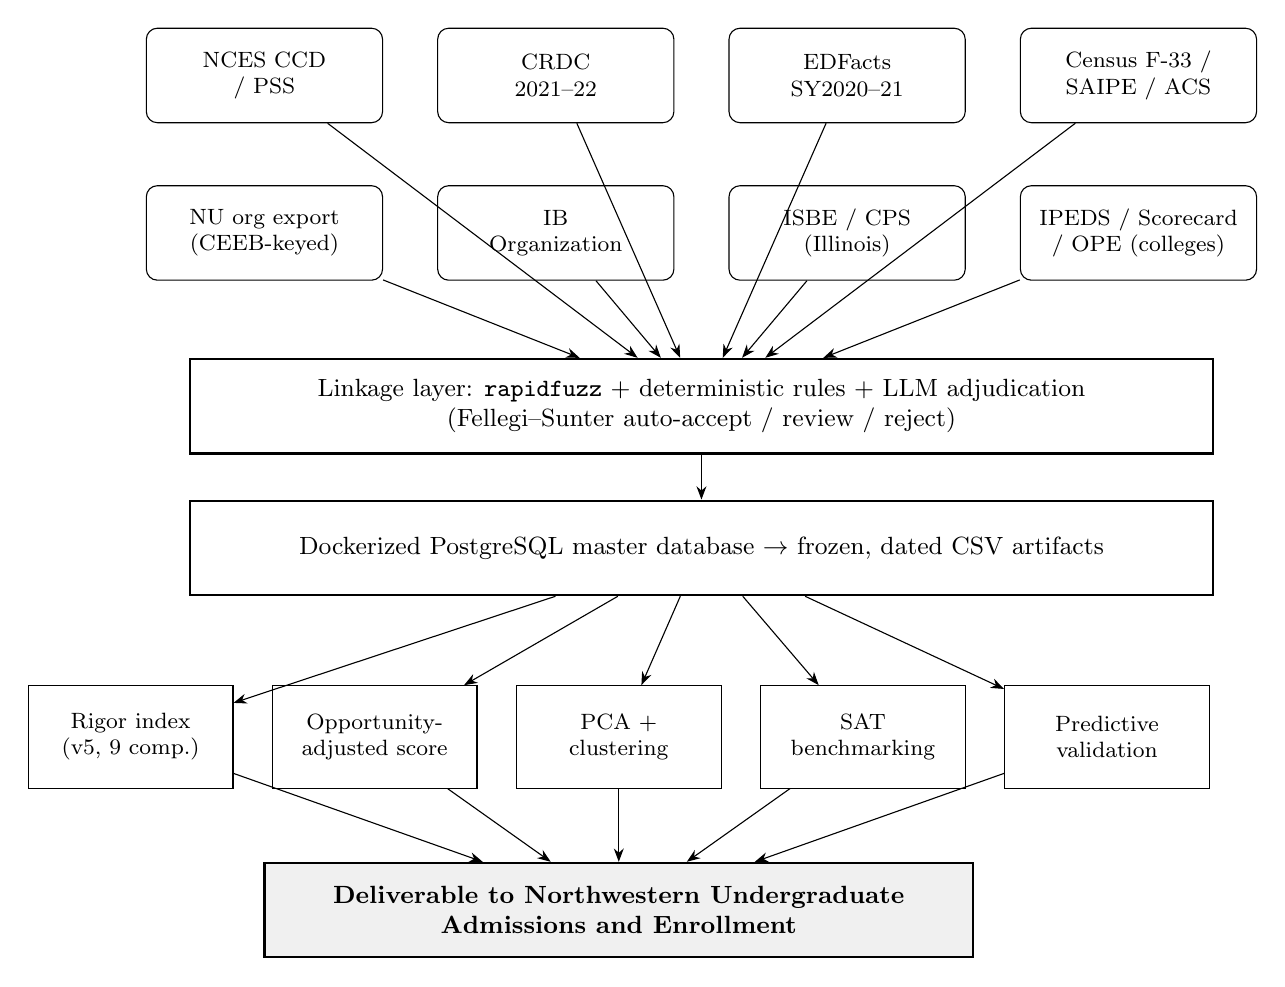
\begin{tikzpicture}[
  src/.style={rectangle, draw, rounded corners, align=center, minimum width=3.0cm, minimum height=1.2cm, inner sep=3pt, font=\footnotesize},
  proc/.style={rectangle, draw, thick, align=center, minimum width=13cm, minimum height=1.2cm, inner sep=4pt, font=\small},
  analysis/.style={rectangle, draw, align=center, minimum width=2.6cm, minimum height=1.3cm, inner sep=3pt, font=\footnotesize},
  deliverable/.style={rectangle, draw, thick, fill=gray!12, align=center, minimum width=9cm, minimum height=1.2cm, inner sep=4pt, font=\small\bfseries},
  >=Stealth
]
\node[src] (s1) at (0,8.4)    {NCES CCD\\/ PSS};
\node[src] (s2) at (3.7,8.4)  {CRDC\\2021--22};
\node[src] (s3) at (7.4,8.4)  {EDFacts\\SY2020--21};
\node[src] (s4) at (11.1,8.4) {Census F-33 /\\SAIPE / ACS};
\node[src] (s5) at (0,6.4)    {NU org export\\(CEEB-keyed)};
\node[src] (s6) at (3.7,6.4)  {IB\\Organization};
\node[src] (s7) at (7.4,6.4)  {ISBE / CPS\\(Illinois)};
\node[src] (s8) at (11.1,6.4) {IPEDS / Scorecard\\/ OPE (colleges)};

\node[proc] (link) at (5.55,4.2) {Linkage layer: \texttt{rapidfuzz} + deterministic rules + LLM adjudication\\(Fellegi--Sunter auto-accept / review / reject)};
\node[proc] (db) at (5.55,2.4) {Dockerized PostgreSQL master database $\rightarrow$ frozen, dated CSV artifacts};

\node[analysis] (a1) at (-1.7,0) {Rigor index\\(v5, 9 comp.)};
\node[analysis] (a2) at (1.4,0)  {Opportunity-\\adjusted score};
\node[analysis] (a3) at (4.5,0)  {PCA +\\clustering};
\node[analysis] (a4) at (7.6,0)  {SAT\\benchmarking};
\node[analysis] (a5) at (10.7,0) {Predictive\\validation};

\node[deliverable] (client) at (4.5,-2.2) {Deliverable to Northwestern Undergraduate\\Admissions and Enrollment};

\foreach \s in {s1,s2,s3,s4,s5,s6,s7,s8} { \draw[->] (\s) -- (link); }
\draw[->] (link) -- (db);
\foreach \a in {a1,a2,a3,a4,a5} { \draw[->] (db) -- (\a); }
\foreach \a in {a1,a2,a3,a4,a5} { \draw[->] (\a) -- (client); }
\end{tikzpicture}%
}
\caption{Data architecture. Sources are linked through a Fellegi--Sunter accept/review/reject decision rule into a Dockerized master database, which feeds five analytical components.}
\label{fig:pipeline}
\end{figure}

\subsection{Linkage design}

No shared identifier exists between the federal school roster (NCES) and the client's roster (CEEB), nor between CEEB and the federal college identifiers. Both junctions were built as Fellegi--Sunter decision rules with three outcomes rather than two, so ambiguous pairs route to clerical review instead of being silently accepted or dropped. Names are normalized before comparison --- generic tokens stripped, abbreviations expanded, truncated client-side names repaired --- then compared with \texttt{rapidfuzz} token ratios blocked on state, with city agreement and, where coordinates exist, haversine distance as corroborating evidence. Because a wrong link is more damaging to an admissions officer than a missing one, different-city pairs reject by default unless one city name contains the other.

The review tier was too large for single-reviewer sign-off, so it was resolved by a three-stage funnel: deterministic rules first, then a large language model \citep{anthropic_claude} adjudicating the residue with original similarity scores retained so any decision can be revisited, and finally hand review of the private-school IB match, whose small universe made full manual adjudication practical.

% ---------------------------------------------------------------------
% METHODS
% ---------------------------------------------------------------------
\section{Methods}
\label{sec:methods}

\subsection{The rigor index}
\label{sec:methods-rigor}

The rigor tier is a transparent weighted composite cut into five ordinal classes, not a supervised classifier; no ground-truth rigor labels exist anywhere in this project. It has four layers, and Appendix~\ref{app:v5} gives the full component specification.

\emph{Layer 0, derived inputs.} AP qualifying density replaces the raw mean exam score as the performance measure. With $t_i$ AP tests taken per student and $\bar{s}_i$ the school's mean exam score, $\mathrm{QD}_i = t_i \cdot \Phi((\bar{s}_i - 2.5)/1.2)$ is the expected number of exams per student scoring 3 or above. A mean score rewards gatekeeping --- a school that sits only its strongest students posts a high mean, while an open-access school is penalized for breadth --- whereas density fuses opportunity with performance. The within-school standard deviation of 1.2 is a documented approximation, since the College Board publishes no school-level score distributions. IB intensity is CRDC IB enrollment over grade 9--12 enrollment, falling back to a verified binary flag; text bands in the client export are mapped to interval midpoints; continuous inputs are winsorized at the 1st and 99th percentiles.

\emph{Layers 1 and 2, standardization and components.} Each sub-feature is $z$-scored across all schools reporting it, with no imputation at any point. Nine components span the client's stated rigor factors, with weights given in Appendix~\ref{app:v5}; each component score is the mean of the $z$-scored sub-features the school actually reports.

\emph{Layer 3, weighted composite with proportional reallocation.} Let $A_i$ be the components available for school $i$ and $\omega_i = \sum_{k \in A_i} w_k$ the share of index weight present. Then
\[
R_i = \frac{\sum_{k \in A_i} w_k\, C_{ik}}{\omega_i}, \qquad \text{defined only where } \omega_i \geq 0.25 .
\]
The coverage floor is the correction that most changed behavior: without it, a school reporting one component with nominal weight 0.05 still received a tier, and its score was a single $z$-score divided by itself. Schools below the floor are logged as unscored and never defaulted to a middle tier.

\emph{Layer 4, tiering.} Tiers are cut by Jenks natural breaks, computed as one-dimensional $k$-means with $k = 5$ and a fixed seed \citep{jenks1967,fisher1958}. An equal-frequency quintile assignment is emitted alongside as a cut-point sensitivity check, and a within-sector track re-tiers inside each sector separately. Following \citet{glaser1963} and \citet{cizek2007}, the tiers are explicitly norm-referenced: a school is ``Most Demanding'' because it sits at the top of this scored population, not because it cleared a fixed external bar.

\subsection{Weight diagnostics, sensitivity, and the opportunity-adjusted score}

Following \citet{cadre2024}, effective weights are computed by variance decomposition on the full-coverage subset and reported alongside nominal weights. Sensitivity is reported under four alternate weighting schemes, twice each --- Jenks refit and cut-points frozen --- because refitting conflates schools moving in the distribution with the boundaries themselves moving. A CRDC-loss scenario zeroes the three CRDC-dependent components to quantify the largest external dependency.

Because the index rewards well-resourced schools while the client's gap-detection goal targets under-resourced ones, a second measure is emitted rather than compromising the first. The rigor score is regressed on socioeconomic context --- district child poverty and free-and-reduced-lunch rate --- and the residual $\tilde{R}_i = R_i - \hat{R}_i$ retained, with schools above its 90th percentile flagged as overperformers. The two measures answer different questions: $R$ asks how demanding a school is, and $\tilde{R}$ asks which schools outperform their circumstances.

\subsection{Feature engineering, clustering, benchmarking, and validation}

Clustering deliberately excludes the rigor score as an input, so that whether recovered clusters reproduce the rigor ordering can be tested rather than assumed. It runs on the raw ingredients --- AP opportunity, CRDC coursework, test participation, graduation rate --- plus region indicators, funding, and poverty; raw coordinates were dropped after client feedback that Euclidean distance over latitude and longitude is not interpretable. Features are $z$-scored, reduced by principal component analysis to the components retaining at least 90 percent of cumulative variance, and partitioned by $k$-means \citep{macqueen1967} in scikit-learn \citep{pedregosa2011}, with $k$ chosen by the gap statistic under the one-standard-error rule \citep{tibshirani2001} and cross-checked against silhouette scores \citep{rousseeuw1987} and a Ward hierarchical partition \citep{ward1963} compared by adjusted Rand index. Clustering is complete-case, and the resulting coverage is reported rather than concealed. Benchmarking computes each school's percentile rank on mean SAT within three peer groups --- region, funding quartile, and rigor tier --- descriptively, with the SAT--poverty correlation alongside so the benchmark's own confounding is visible.

Predictive validation implements the literature's own test of a rigor construct: Adelman built a curriculum-intensity index and then regressed degree completion on it. Here the four-year adjusted cohort graduation rate is regressed on three nested blocks --- socioeconomic status only, opportunity only, and both --- using ordinary least squares and gradient boosting, with an 80/20 train--test split and permutation importance on the test set. Only opportunity features enter as predictors, since predicting an outcome from other outcomes would be circular, and the claim rests on the incremental $R^2$ rather than on absolute fit. Pipeline validation is separate and must also pass: the pipeline rebuilds from source through \texttt{docker compose up -{}-build} under row-count and schema assertions, with an automated test suite that skips when the gitignored raw sources are absent.

% ---------------------------------------------------------------------
% RESULTS
% ---------------------------------------------------------------------
\section{Results}
\label{sec:results}

\subsection{Identifier linkage}

The school-side junction resolved 5{,}416 public and 290 private review-tier candidate pairs. Deterministic rules settled roughly 88 percent before any model was invoked; the language model judged the remaining 635, accepting 232 public and 12 private. Final tiers were 14{,}096 accept and 10{,}087 reject on the public side and 550 accept, 803 reject, and 1 review on the private side --- a net gain of 2{,}460 public and 40 private schools with a usable CEEB code.

Match rates depend entirely on the denominator, so the project reports three rather than one. Of the 25{,}577 verified high schools in the federal roster, 16{,}508 (64.5 percent) carry a confirmed link to a client record; within the frozen modeling dataset, 16{,}111 of the 21{,}832 rows that have a school-side record match (73.8 percent); and 16{,}111 of all 34{,}392 modeling rows carry a link (46.8 percent). The third is a coverage statement, not a match rate, because 12{,}560 modeling rows are organization-only records that cannot match by construction.

A bidirectional audit tested the reverse direction. Of 40{,}359 unique high schools in the client's export, 28{,}301 (70.1 percent) appear in the federally anchored universe; of the federal roster, 21{,}359 (83.5 percent) link to a client record, 81.3 percent at high confidence, leaving 4{,}218 genuinely absent. A geographic audit of 15{,}263 matched public schools with coordinates on both sides found a median discrepancy of 1.0 km and 94.3 percent within 10 km --- independent evidence that the name-based rules are not systematically wrong --- leaving 364 pairs beyond 50 km as a standing quality-assurance list.

The 4{,}218 missing schools are not random. Median enrollment is 39, but 421 enroll 500 or more students, and audit confirmed five suburban schools of 2{,}861 to 4{,}291 students that opened between 2001 and 2003 and are absent while same-district neighbors are present: the client's roster appears never to have back-filled that construction cohort. The list also includes 41 IB schools and 820 schools that already carry a rigor tier.

On the college side, the junction matched 2{,}794 of 4{,}004 college CEEB codes (69.8 percent), of which 2{,}769 linked to College Scorecard. The most consequential engineering detail was format: Scorecard ships OPE identifiers as float-formatted strings, so a naive join matches zero rows, while stripping the decimal and zero-padding to eight digits raised linkage to 98.6 percent. The 1{,}235 unmatched rows are almost entirely institutions that no longer exist under their listed identity --- 875 closed or renamed independents, 129 closed for-profit chains --- a historical artifact of the client's list rather than a matching failure.

\subsection{Coverage is structurally non-random}

A single overall coverage number would mislead. At feature level (Figure~\ref{fig:featcov}), CRDC signals are public-school-only by federal design, so private coverage is exactly zero for AP participation, dual enrollment, test-taker rate, graduation rate, and free-and-reduced-lunch rate; the public test-taker rate reaches 91 percent while the private figure is zero. Client-sourced analytics track the recruiting universe instead: roughly 40 percent of public and 17 percent of private schools.

\begin{figure}[htbp]
\centering
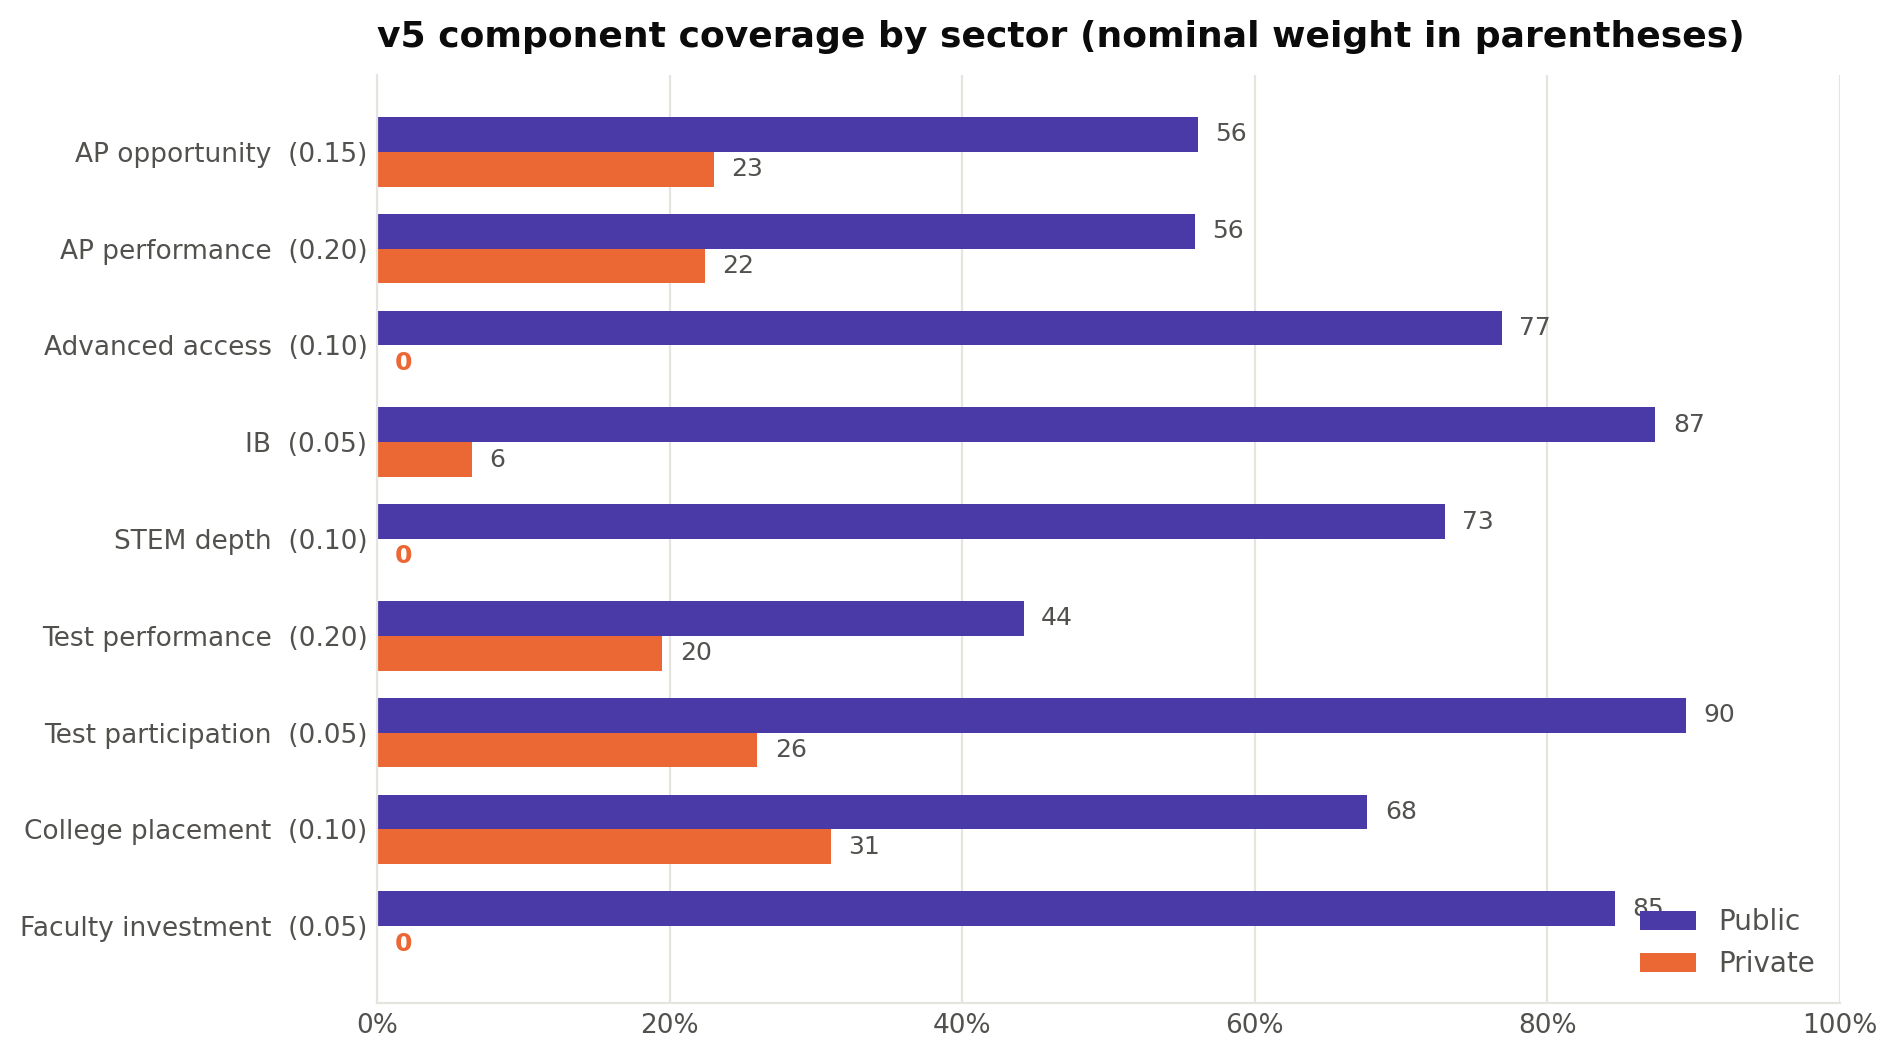
\includegraphics[width=0.80\textwidth]{v5_component_coverage.png}
\caption{Coverage of the nine v5 index components by sector. Advanced access, STEM depth, and faculty investment are zero percent for private schools by federal design, not by matching failure, so a private school is scored on at most six of nine components.}
\label{fig:coverage}
\end{figure}

Figure~\ref{fig:coverage} carries that through to the index. Three of the nine components --- advanced access, STEM depth, and faculty investment --- are zero percent covered for private schools, so a private school is scored on at most six of nine, and after the coverage floor only 3{,}250 of 13{,}229 private schools are tiered at all. The pooled score does not compare like with like. Within-sector standardization changes the picture substantially, placing 1{,}270 private and 1{,}179 public schools in the top tier against a pooled split that strongly favors public schools with full CRDC coverage. Both tracks ship and neither is the default, because whether a private school should be ranked against private peers or nationally is a client decision, not a modeling one.

\subsection{The rigor index: coverage, tiers, weights, and validation}

The index scores 22{,}869 of 45{,}250 organization records (50.5 percent) --- 17{,}015 public and 3{,}250 private. The coverage floor moved the maximum from 7.66 to 3.33, eliminating an artifact in which two schools scored on the IB component alone outranked every school reporting all nine. The cost is explicit: 6{,}167 schools become unscored, most previously tiered on a single band-coded field. Reporting those as measured rigor was not defensible; reporting them as insufficient data is.

Fitted Jenks cut-points are $-0.704$, $-0.207$, $+0.286$, and $+0.977$. Table~\ref{tab:validation} reports tier means against six measures, and the distinction between them matters. The four-year graduation rate is the only fully external validator --- it is never an index input --- and it rises monotonically from 69.8 to 95.5 percent across the tiers. Mean SAT, AP score, college-going rate, and STEM breadth are the untransformed forms of index components, so their monotonicity is an internal consistency check, not independent validation. Child poverty, also not an input, declines monotonically, which makes the entanglement of Section~\ref{sec:ses} visible rather than argued about. Jenks and equal-frequency quintile schemes agree on only 58.4 percent of scored schools, so the cut-point choice is consequential rather than cosmetic.

\begin{table}[htbp]
\centering
\singlespacing\small
\caption{Rigor tier means against six measures. Graduation rate and child poverty are not index inputs; the other four are untransformed forms of index components and are reported as an internal consistency check.}
\label{tab:validation}
\setlength{\tabcolsep}{4.5pt}
\begin{tabular}{@{}lrrrrrrr@{}}
\toprule
Tier & $n$ & Grad.\ rate & Mean SAT & AP score & \% to college & STEM breadth & Child poverty \\
\midrule
Below Average   & 2{,}868 & 69.8 & 1{,}041 & 1.79 & 35.6 & 1.20 & 18.2 \\
Average         & 7{,}299 & 85.6 & 1{,}099 & 2.20 & 51.3 & 2.93 & 17.3 \\
Demanding       & 7{,}211 & 89.7 & 1{,}139 & 2.66 & 64.1 & 3.54 & 14.2 \\
Very Demanding  & 4{,}050 & 92.3 & 1{,}178 & 3.08 & 74.2 & 3.76 & 12.6 \\
Most Demanding  & 1{,}441 & 95.5 & 1{,}252 & 3.47 & 85.9 & 3.81 & 12.0 \\
\bottomrule
\end{tabular}
\end{table}

Table~\ref{tab:weights} reports the diagnostic the composite-indicator literature demands. AP performance contributes 0.364 of index variance against a designed weight of 0.20, nearly twice its nominal share, while test participation contributes 0.015 against a nominal 0.05. This is direct empirical confirmation of Section~\ref{sec:academic-rigor}: performance carries the signal, and participation, correlated with everything else, is largely absorbed. STEM depth and faculty investment also under-contribute, being low-variance measures --- STEM breadth is a 0--4 integer where 73 percent of public schools sit at 3 or 4, and teacher certification is 100 percent at the median school. They earn their place by covering client factors nothing else addresses, not by discriminating strongly.

\begin{table}[htbp]
\centering
\singlespacing\small
\caption{Nominal versus effective weights, by variance decomposition on the 5{,}604 full-coverage schools.}
\label{tab:weights}
\begin{tabular}{@{}lrr@{}}
\toprule
Component & Nominal & Effective \\
\midrule
AP opportunity      & 0.15 & 0.129 \\
AP performance      & 0.20 & \textbf{0.364} \\
Advanced access     & 0.10 & 0.096 \\
IB                  & 0.05 & 0.017 \\
STEM depth          & 0.10 & 0.031 \\
Test performance    & 0.20 & \textbf{0.247} \\
Test participation  & 0.05 & 0.015 \\
College placement   & 0.10 & 0.079 \\
Faculty investment  & 0.05 & 0.022 \\
\bottomrule
\end{tabular}
\end{table}

Under equal weighting the score correlates with the shipped index at Spearman $\rho = 0.950$, and under a performance-heavy scheme at $\rho = 0.959$. Against the prior specification, $\rho = 0.879$ and 32.3 percent of schools change tier on score movement alone with cut-points frozen. Two readings follow. Which components are in the index is load-bearing --- adding exam-performance signal to an availability-only specification moves about a third of schools across tiers --- while the weights themselves largely are not. The honest counterpoint is that a composite whose tier boundaries move roughly a quarter of schools under any plausible re-weighting carries genuine specification uncertainty, which is why the tier ships decomposable rather than as a single opaque number.

Zeroing the three CRDC-dependent components among the 11{,}290 schools that carry CRDC signal yields $\rho = 0.958$ but changes 40.5 percent of tier assignments. CRDC access is the single largest external dependency, and given the delays documented in Section~\ref{sec:literature-review}, this is the fragility most worth putting in front of the client.

\subsection{Socioeconomic entanglement and the opportunity-adjusted score}
\label{sec:ses}

The check the literature demands returns an unfavorable answer, reported as such. The rigor score's Spearman correlation with district child poverty is $-0.323$, up from $-0.168$ under the previous specification, and the increase is concentrated where theory predicts: test performance ($-0.392$) and AP performance ($-0.391$) are the most entangled components, IB ($-0.047$) and test participation ($+0.044$) the least. This is the measurable cost of the shift toward exam performance, visible in Table~\ref{tab:validation} as well, where child poverty declines monotonically across tiers.

The opportunity-adjusted residual is the remedy. Socioeconomic context explains $R^2 = 0.209$ of the score across 19{,}150 schools, and the residual's correlation with poverty is $-0.028$, effectively zero. The raw tier places 69 high-poverty schools in the top tier; the residual surfaces 343 high-need overperformers, a fivefold increase, and named examples pass inspection --- Bronx High School of Science, Brooklyn Technical, Julia R. Masterman in Philadelphia, Metro High in St.\ Louis, and Eleanor Roosevelt in New York.

A related lens, requested by the client, is AP efficiency: $z(\text{AP exam score}) - z(\text{AP tests offered})$, computed on the 10{,}504 schools with both signals. It isolates 1{,}597 ``selective and effective'' schools --- few offerings, strong exam outcomes --- of which only 4 reach the top tier, because a thin AP catalog drags an additive composite down even when students perform as well as schools two tiers higher (Figure~\ref{fig:apeff}). For the recruiting question of where strong students emerge from limited resources, this flag is arguably more actionable than the tier, and it ships alongside the tier rather than folded into it.

\subsection{Clustering}

Clustering ran on the 5{,}837 of 34{,}392 schools (17.0 percent) with complete data across every feature. Six principal components retained roughly 92 percent of cumulative variance; the first loads on funding (0.79) against poverty ($-0.48$), with the Northeast positive and the South negative.

The gap statistic selected $k = 8$. The silhouette score at that solution is 0.182, below the conventional 0.25 threshold, and the adjusted Rand index between the $k$-means and Ward partitions is 0.353. Per the validation plan this is reported as a finding about the data: the population has weak natural cluster separation, and plausible groups blur rather than forming tight regions. Table~\ref{tab:clusters} nonetheless shows interpretable structure, and 26.3 percent of rigor-tier variance sits between clusters --- real alignment with the independently computed tier, but far from complete. Cluster 3 is a well-funded, high-rigor Northeastern group, cluster 0 reaches comparable rigor in the South on participation rather than funding, and clusters 1 and 5 are the under-resourced end.

The college-side clustering behaves the same way: silhouette favors $k = 2$, recovering the public two-year versus private four-year divide, so a fixed six-cluster solution is emitted alongside as operational segments. Selectivity measures are reported as profile overlays rather than clustering inputs, since open-admission and two-year institutions are exempt from those IPEDS components and coverage is only 42 to 62 percent.

\subsection{Benchmarking and predictive validation}

Mean SAT rises monotonically across the rigor tiers on the modeling-track population --- 1{,}068, 1{,}127, 1{,}168, 1{,}232, 1{,}287, a 219-point spread with no inversions --- though SAT is itself an index component, so this is consistency rather than independent validation. Two measures deliberately held out of that index validate it only partly. Graduation rate separates the bottom tier sharply (71.0 percent against 86 to 89 percent above it) but saturates, dipping to 84.7 percent in the small top tier; advanced-STEM breadth rises 3.04 to 3.41 through the first four tiers and dips at the fifth. Both patterns are consistent with a top tier defined by exam performance rather than catalog breadth --- the phenomenon the AP-efficiency lens isolates --- and are reported rather than smoothed. The accompanying check matters more: SAT correlates with child poverty at $\rho = -0.385$ here, roughly three times the rigor tier's own entanglement, so an outcome measure is more socioeconomically confounded than an opportunity-plus-performance measure. The benchmark is also composite-level only, which averages sub-scores of very different predictive validity and income sensitivity \citep{geiser_studley2002,bettinger2013}.

Predictive validation (Figure~\ref{fig:predictive}) returns a modest but stable result. On the main specification ($n = 1{,}691$), a socioeconomic-only baseline reaches $R^2 = 0.370$ under ordinary least squares and 0.373 under gradient boosting, opportunity-only reaches 0.214 and 0.230, and the combined model reaches 0.420 and 0.428 --- an increment of $+0.050$ and $+0.055$. On the CRDC-only specification, which avoids recruiting-universe selection bias entirely ($n = 6{,}158$), the increment is $+0.035$ and $+0.067$. Permutation importance is dominated by the free-and-reduced-lunch rate (0.506), followed by CRDC AP participation (0.066) and test-taker rate (0.050).

Two readings follow. Opportunity structure carries real incremental signal beyond socioeconomic status, stable across two very different specifications and both model families, so the index measures something rather than re-describing demographics. But socioeconomic status remains the dominant predictor of graduation --- the honest companion to the entanglement result above. Linear and boosted models tie on the same rows; the boosted model's advantage appears only when exploiting the larger missing-data universe, reaching $R^2 = 0.517$ across all 17{,}420 public schools with a target.

% ---------------------------------------------------------------------
% DISCUSSION
% ---------------------------------------------------------------------
\section{Discussion}
\label{sec:discussion}

The composite-indicator literature predicted that a levels-based school index would reproduce socioeconomic ordering, and it does. At $\rho = -0.323$ with child poverty the rigor score is not a poverty proxy, but it is measurably entangled, and the entanglement grew as the index improved along the dimension the rigor literature demanded. Any index that follows \citet{geiser2004} toward exam performance buys predictive validity with socioeconomic confounding: the two goals are in tension by construction, not by poor implementation.

The resolution matters more than the finding. Rather than compromising the rigor measure to make it look fairer, the platform emits a second, orthogonal measure uncorrelated with poverty that surfaces five times as many high-need overperformers. Two measures answering two questions, rather than one answering neither well, is this paper's main transferable contribution, and it is what the 2019 adversity-score episode should have taught the field. The AP-efficiency lens applies the same idea to one component: 1{,}597 schools do a great deal with a thin AP catalog, and an additive composite hides them.

The predictive-validation result should temper claims made to any client. Opportunity structure adds only 0.04 to 0.05 in $R^2$ over socioeconomic status, and the dominance of the free-and-reduced-lunch rate in permutation importance is a reminder that school-level outcomes are heavily determined by student composition. A rigor tier is defensible as a description of what a school offers and how its students perform on it, not as a prediction about an individual applicant --- and the tier labels, which retain the client's counselor vocabulary, invite exactly that misreading.

The clustering result is negative and is reported as such. A silhouette of 0.182, an adjusted Rand index of 0.353, and 17 percent complete-case coverage together say that American high schools do not separate into tight types on these features. That argues against a typology product and in favor of the continuous, decomposable index --- though it would have been easy to present eight labeled clusters as discovered structure instead.

Finally, the linkage work produced a finding neither party expected. The residue that fails to match in both junctions is not a matching failure but a historical artifact of the client's own reference data. A crosswalk built for one purpose became an audit of that data, and the 4{,}218 missing schools are directly actionable for recruiting.

% ---------------------------------------------------------------------
% CONCLUSIONS
% ---------------------------------------------------------------------
\section{Conclusions}
\label{sec:conclusion}

This project delivered a working, internally owned replacement for the school-context capability that disappeared with Landscape. Sixteen public sources and the client's own export were consolidated into a Dockerized database and two frozen analytical universes; schools and colleges were linked across three identifier systems under a Fellegi--Sunter decision rule with an auditable trail on every accepted match; and a nine-component rigor index was built, tiered, weight-audited, sensitivity-tested, and validated against five external measures it was not built from.

Three findings stand out. Measured effective weights diverge sharply from designed weights, with AP exam performance contributing 0.364 of index variance against a nominal 0.20 --- empirical confirmation that performance rather than availability carries the signal. The index reproduces socioeconomic ordering at $\rho = -0.323$, which motivated a second orthogonal measure uncorrelated with poverty that surfaces five times as many high-need overperformers. And opportunity structure predicts graduation beyond socioeconomic status by only 0.04 to 0.05 in $R^2$, which bounds how strong a claim the tier can support.

Three results are deliberately negative. Clustering is weak by conventional standards and is reported as a property of the data. Private schools cannot be scored on the same instrument as public schools, since three of nine components are zero percent covered for them by federal design, so the platform ships a pooled and a within-sector track. And losing CRDC access would change 40.5 percent of tier assignments among schools carrying CRDC signal --- a live risk, given that the collection is six months late and its office is being relocated.

The project also corrected three assumptions in its own plan: that no public source publishes school-level AP participation, that no governmental considerations apply to a tool of this kind, and that the federal statistical infrastructure underneath it is stable. The first opened a data source, the second belongs in front of the client and the university's counsel, and the third is why every artifact here is frozen and dated.

% ---------------------------------------------------------------------
% LIMITATIONS AND FUTURE WORK
% ---------------------------------------------------------------------
\section{Limitations and Future Work}
\label{sec:future-work}

Four limitations bound every result above. The tier is norm-referenced, so cut-points shift if the scored population changes, and that population is roughly half the client's universe and skews toward the recruiting footprint. The AP qualifying-density measure assumes a within-school score standard deviation of 1.2, an approximation per-course distributions would replace with a measurement. The graduation-rate target is a COVID-affected cohort, privacy-blurred and compressed near its ceiling, so the $R^2$ figures have structural ceilings. And no ground-truth rigor labels exist, so Table~\ref{tab:validation} is convergent evidence, not accuracy.

Four extensions are scoped. Term-frequency--inverse-document-frequency token weighting would down-weight the uninformative tokens that saturate school names, the cheapest improvement to the auto-accept rate \citep{cohen2003}. An expectation-maximization Fellegi--Sunter implementation would return calibrated match probabilities rather than similarity scores, and validated matches would be contributed back upstream \citep{enamorado2019,binette2022,ucboulder_crosswalk}. Rerunning predictive validation on a post-COVID graduation vintage would remove the target's largest caveat, and extending the junction to a historical IPEDS year would recover the renamed-institution residue.

Two decisions remain with the client: whether private schools are tiered against private peers or nationally, and whether the 48 correctional facilities now flagged should be excluded outright.

% ---------------------------------------------------------------------
% AVAILABILITY
% ---------------------------------------------------------------------

% ---------------------------------------------------------------------
% REFERENCES
% ---------------------------------------------------------------------
\newpage
\singlespacing
\printbibliography[title={References}]
\addcontentsline{toc}{section}{References}
\doublespacing

% ---------------------------------------------------------------------
% APPENDICES
% ---------------------------------------------------------------------
\newpage
\appendix
\singlespacing

\section{Glossary of Identifiers and Acronyms}
\label{app:glossary}

{\small
\begin{longtable}{@{}ll@{}}
\toprule
Acronym & Meaning \\
\midrule
\endfirsthead
\toprule
Acronym & Meaning \\
\midrule
\endhead
NCES & National Center for Education Statistics \\
CCD & Common Core of Data (NCES public school universe) \\
PSS & Private School Universe Survey (NCES) \\
ELSI & Elementary/Secondary Information System (NCES extraction tool) \\
CEEB & College Entrance Examination Board school code \\
OPE / OPEID & Office of Postsecondary Education identifier \\
UNITID & IPEDS institutional survey key \\
IPEDS & Integrated Postsecondary Education Data System \\
CRDC & Civil Rights Data Collection \\
EDFacts & U.S. Department of Education school-level reporting collection \\
ACGR & Four-year adjusted cohort graduation rate \\
SAIPE & Small Area Income and Poverty Estimates (Census) \\
F-33 & Annual Survey of School System Finances (Census) \\
ACS & American Community Survey (Census) \\
LEAID & Local Education Agency identifier (district join key) \\
FRL & Free and reduced-price lunch eligibility rate \\
AP & Advanced Placement (College Board) \\
IB / IBDP & International Baccalaureate / IB Diploma Programme \\
NAEP & National Assessment of Educational Progress \\
SEDA & Stanford Education Data Archive \\
ISBE & Illinois State Board of Education \\
CPS & Chicago Public Schools \\
PCA & Principal component analysis \\
ARI & Adjusted Rand index \\
TF-IDF & Term frequency--inverse document frequency \\
\bottomrule
\end{longtable}}\addtocounter{table}{-1}

\clearpage
\section{Source Inventory and Vintages}
\label{app:sources}

Vintages are those actually consumed by the frozen artifacts, not the publisher's current release. \emph{Accessed} is the earliest date the file is demonstrably present in the project repository, derived from git history by \texttt{etl/data\_provenance.py} rather than self-reported. Each source is cited in Section~\ref{sec:data} and listed in the references.

{\small\raggedright
\begin{longtable}{@{}p{3.1cm}p{2.2cm}p{2.3cm}p{4.7cm}@{}}
\toprule
Source & Vintage & Accessed & Contribution \\
\midrule
\endfirsthead
\toprule
Source & Vintage & Accessed & Contribution \\
\midrule
\endhead
NCES CCD & current release & 2026-06-26 & Public school universe, enrollment, locale \\
NCES PSS & current release & 2026-07-02 & Private school universe (49-state merge) \\
NCES ELSI & current release & 2026-07-05 & Extraction tool; 12-digit NCESSCH re-pull \\
CRDC & SY 2021--22 & 2026-07-24$^{\dagger}$ & AP, IB, dual enrollment, SAT/ACT, STEM, certification \\
EDFacts & SY 2020--21 & 2026-06-26$^{\dagger}$ & Graduation rate; assessment participation \\
Census F-33 & FY 2024 & 2026-06-26 & District revenue \\
Census SAIPE & 2024 & 2026-06-26 & County and district child poverty \\
Census ACS & 2020--2024 & 2026-07-20 & County neighborhood context \\
NAEP & 2024 & 2026-06-26 & National and state context (not school grain) \\
College Board AP & 2024--25 & 2026-06-26 & National and state aggregates only \\
IB Organization & 2025--26 scrape & 2026-06-28 & IB World School directory \\
ISBE Report Card & 2025 & 2026-06-26 & Illinois ACT and per-pupil expenditure \\
CPS Opportunity Index & SY 2026 & 2026-06-26 & Chicago pilot region \\
IPEDS HD2023 & 2023 & 2026-08-01 & College geography and Carnegie level \\
College Scorecard & 2023--24 & 2026-08-02$^{\dagger}$ & College outcomes and price \\
OPE ID & n/a & n/a & Identifier system carried inside IPEDS and Scorecard \\
UC Boulder crosswalk & rev.\ 2025-01-06 & 2026-07-06 & NCES-to-CEEB seed, 21{,}391 schools \\
NU organization export & 2026-07-31 & 2026-07-31 & School-level AP, SAT, placement, context \\
\bottomrule
\end{longtable}}\addtocounter{table}{-1}

\noindent $^{\dagger}$ Reaches the project bundled inside the combined schools export rather than as an independent pull, so the date bounds possession rather than recording retrieval.

\clearpage
\section{Supplementary Figures}
\label{app:figures}

Figures~\ref{fig:v5tiers}--\ref{fig:v5sens} are generated from the v5 index tables by
\texttt{etl/build\_rigor\_v5\_figures.py}; Figures~\ref{fig:featcov}--\ref{fig:predictive}
come from the v4 analytical chain by \texttt{etl/build\_rigor\_figures.py}. Both scripts read
only frozen, dated artifacts and reproduce byte-for-byte on re-run.

\begin{figure}[htbp]
\centering
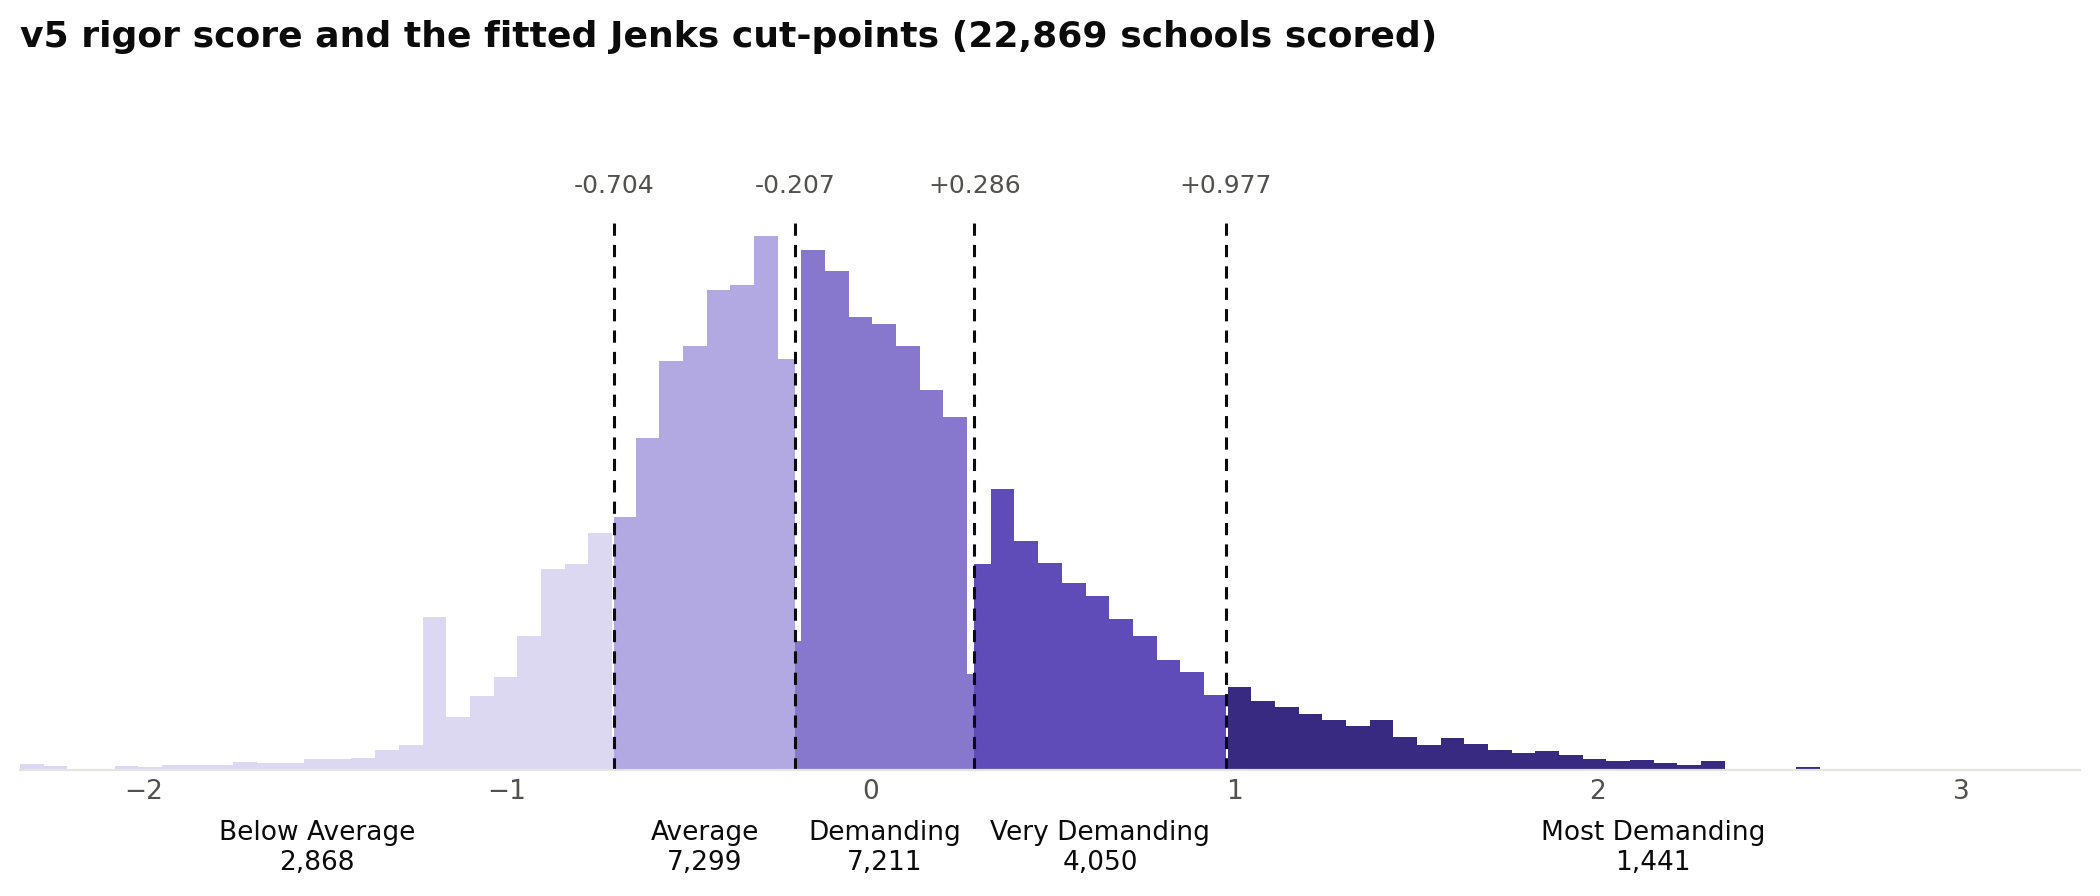
\includegraphics[width=0.92\textwidth]{v5_tiers.png}
\caption{The continuous v5 rigor score with the fitted Jenks cut-points. Natural breaks cut at gaps in the distribution rather than at equal counts, so the tiers are deliberately unequal in size.}
\label{fig:v5tiers}
\end{figure}

\begin{figure}[htbp]
\centering
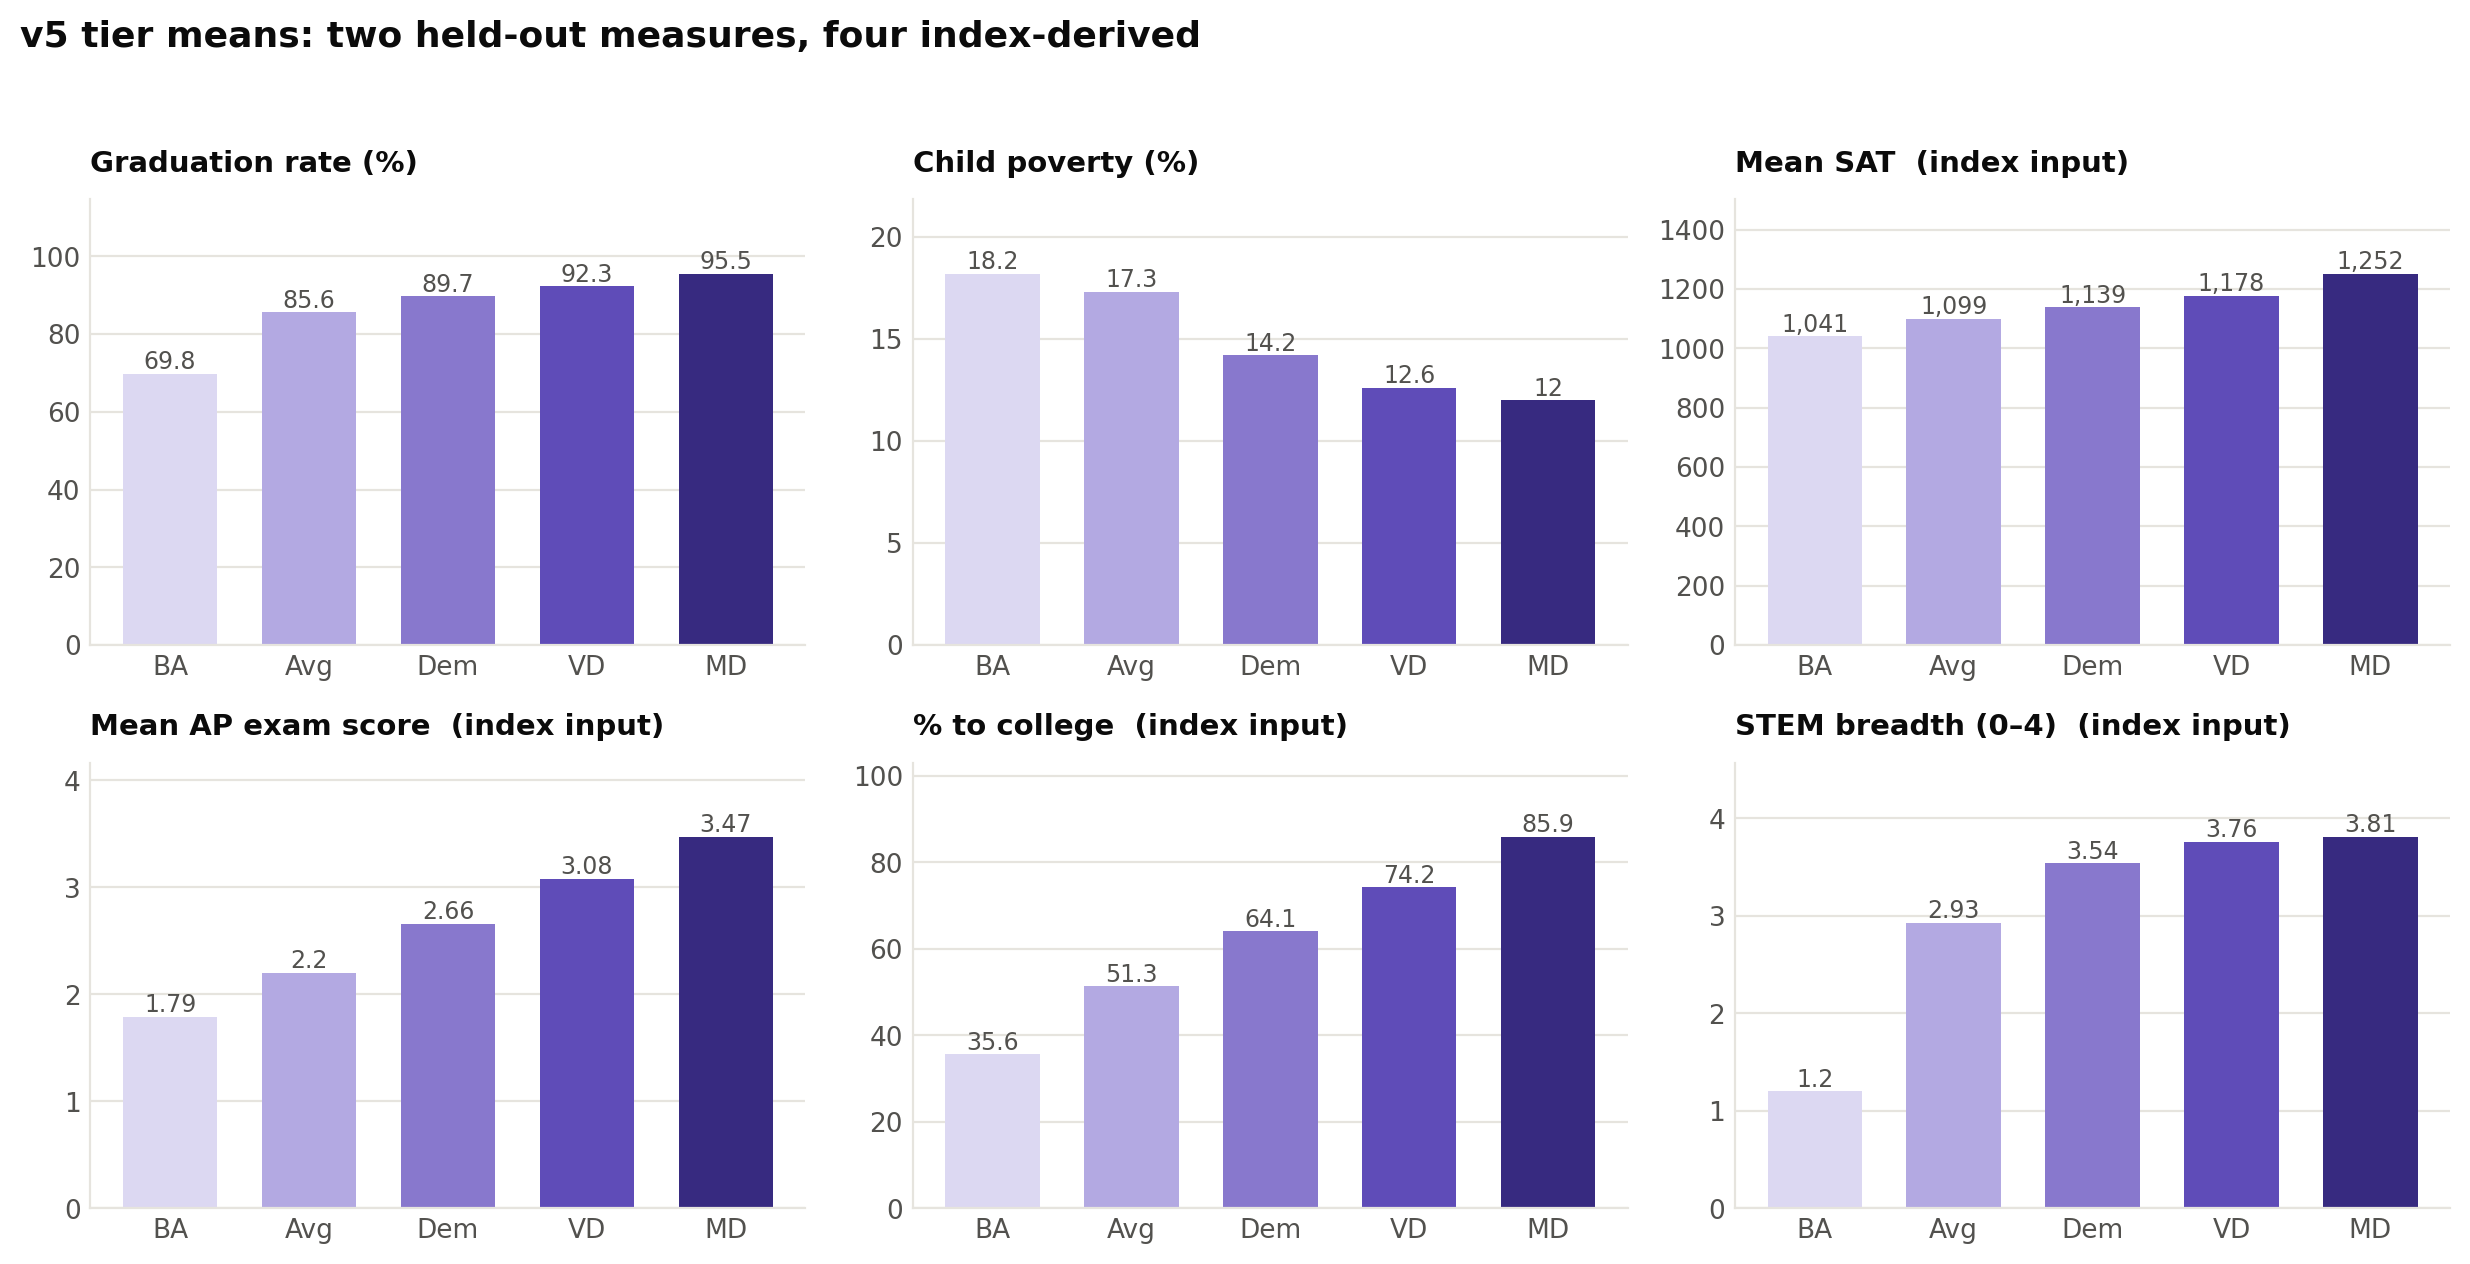
\includegraphics[width=0.94\textwidth]{v5_validation.png}
\caption{Tier means for Table~\ref{tab:validation}. Graduation rate and child poverty are never index inputs; the other four panels are the untransformed forms of index components and are an internal consistency check.}
\label{fig:v5val}
\end{figure}

\begin{figure}[htbp]
\centering
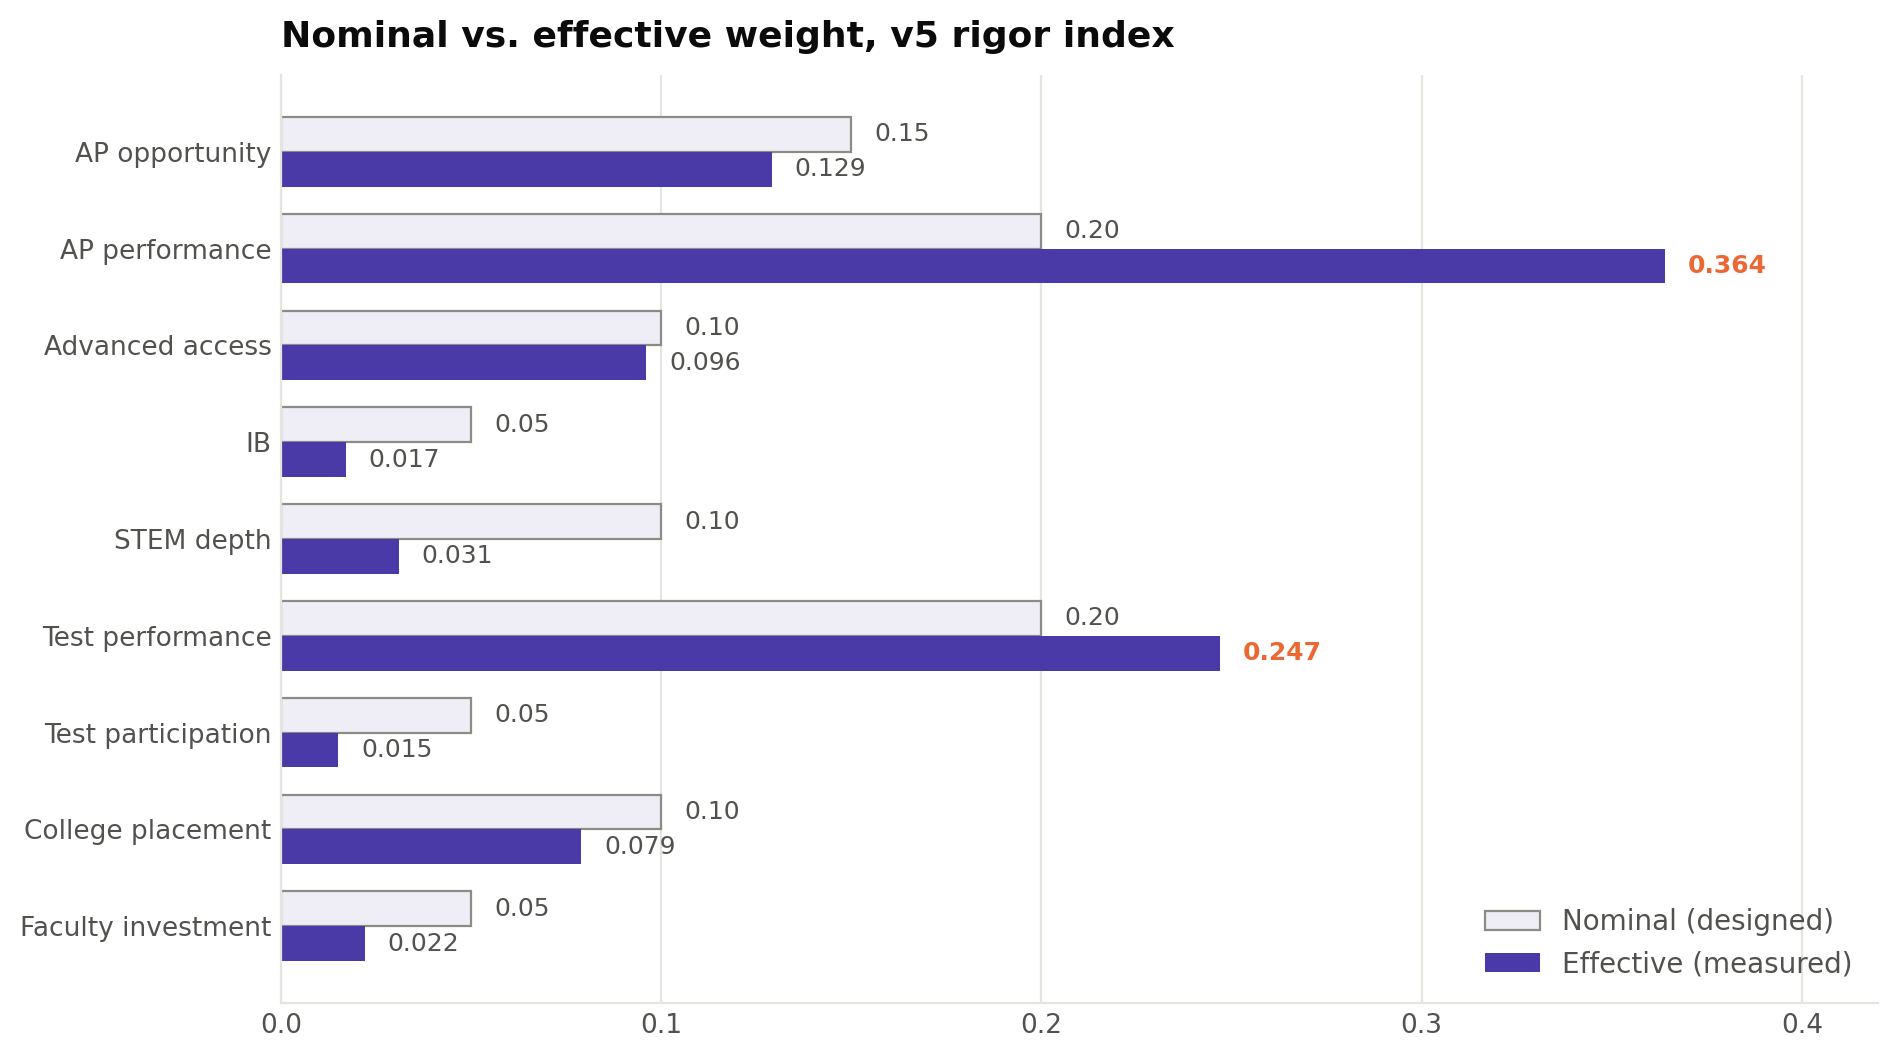
\includegraphics[width=0.86\textwidth]{v5_weights.png}
\caption{Nominal versus effective weight, the numbers in Table~\ref{tab:weights}. AP performance contributes nearly twice the variance it was designed to carry.}
\label{fig:v5wts}
\end{figure}

\begin{figure}[htbp]
\centering
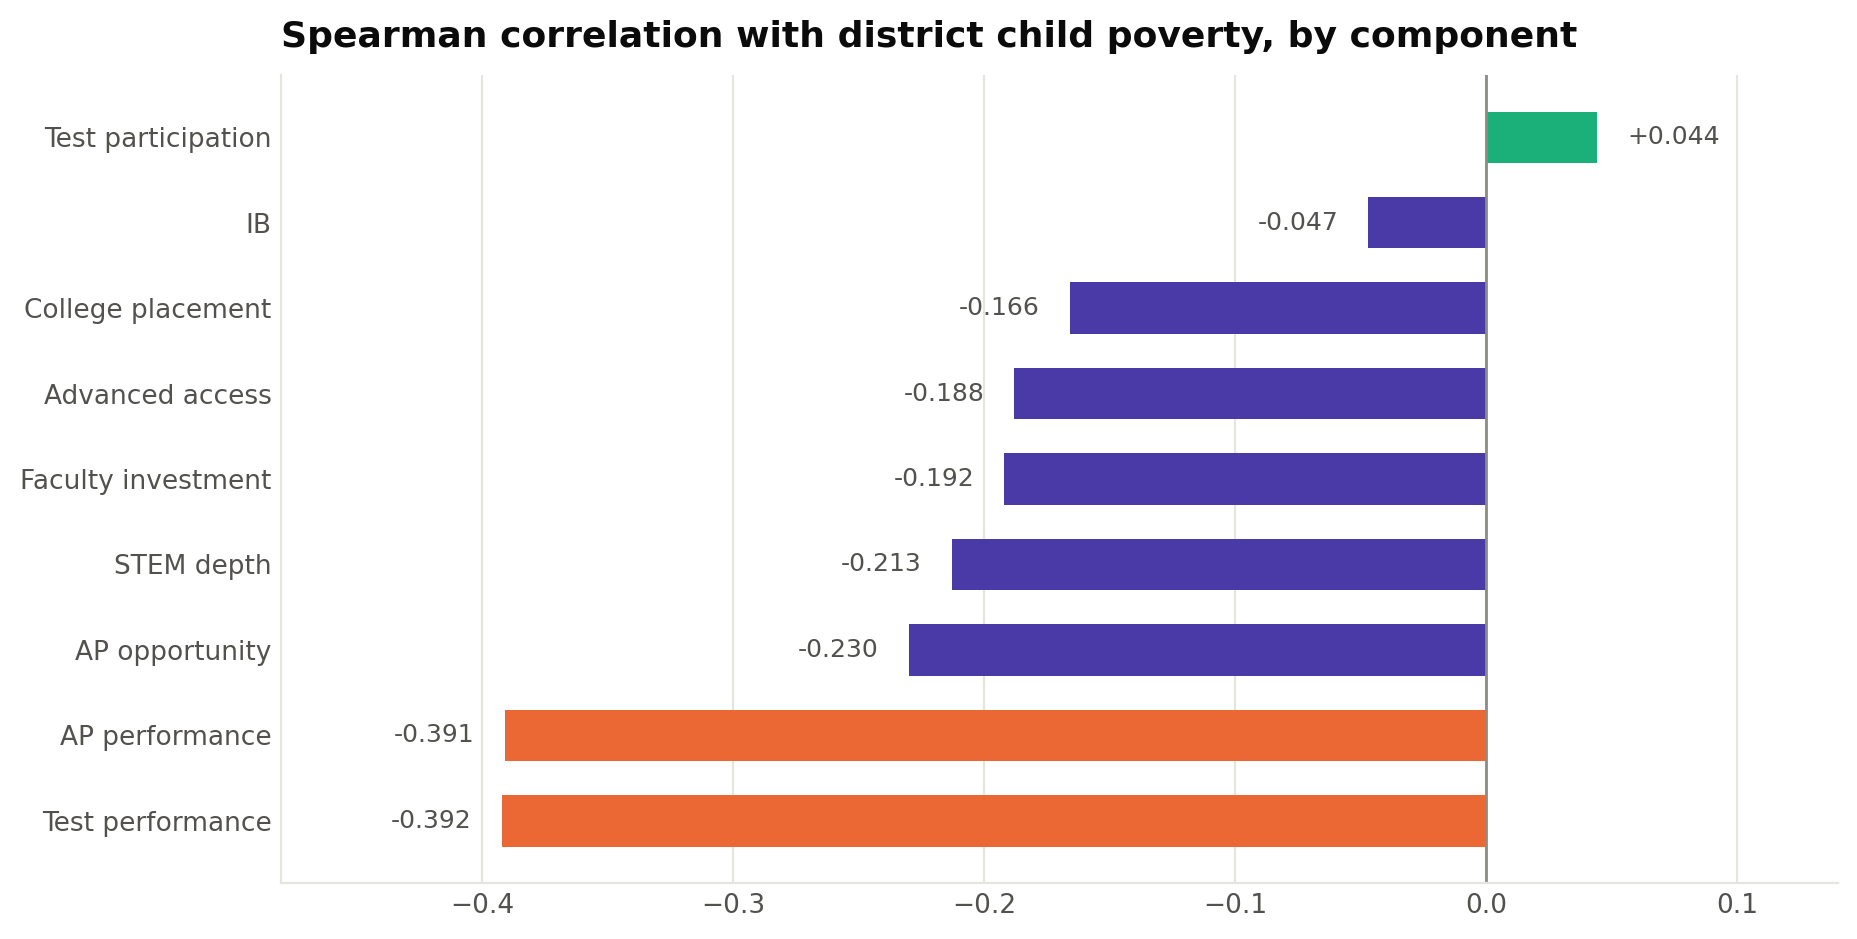
\includegraphics[width=0.86\textwidth]{v5_ses_entanglement.png}
\caption{Where the index's socioeconomic entanglement comes from. The two exam-performance components are the most poverty-correlated; IB and test participation are effectively uncorrelated.}
\label{fig:v5ses}
\end{figure}

\begin{figure}[htbp]
\centering
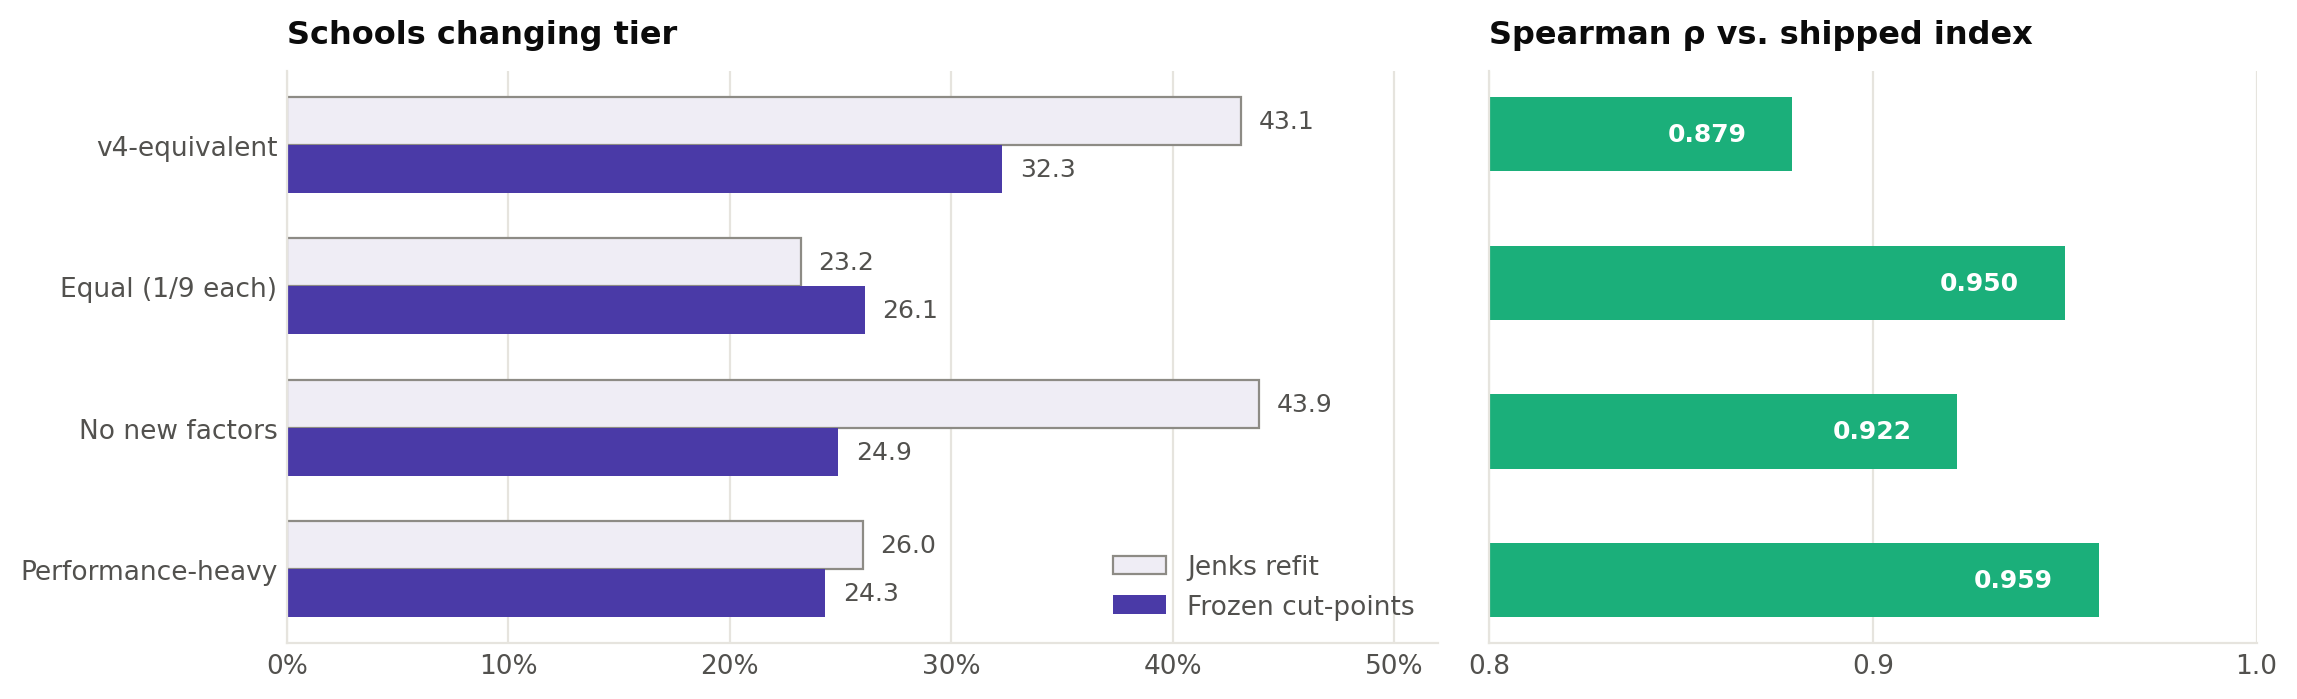
\includegraphics[width=0.98\textwidth]{v5_sensitivity.png}
\caption{Tier movement under alternate weighting schemes, reported on both tiering conventions. Frozen cut-points isolate movement in the score; refitting Jenks conflates that with movement in the boundaries.}
\label{fig:v5sens}
\end{figure}

\begin{figure}[htbp]
\centering
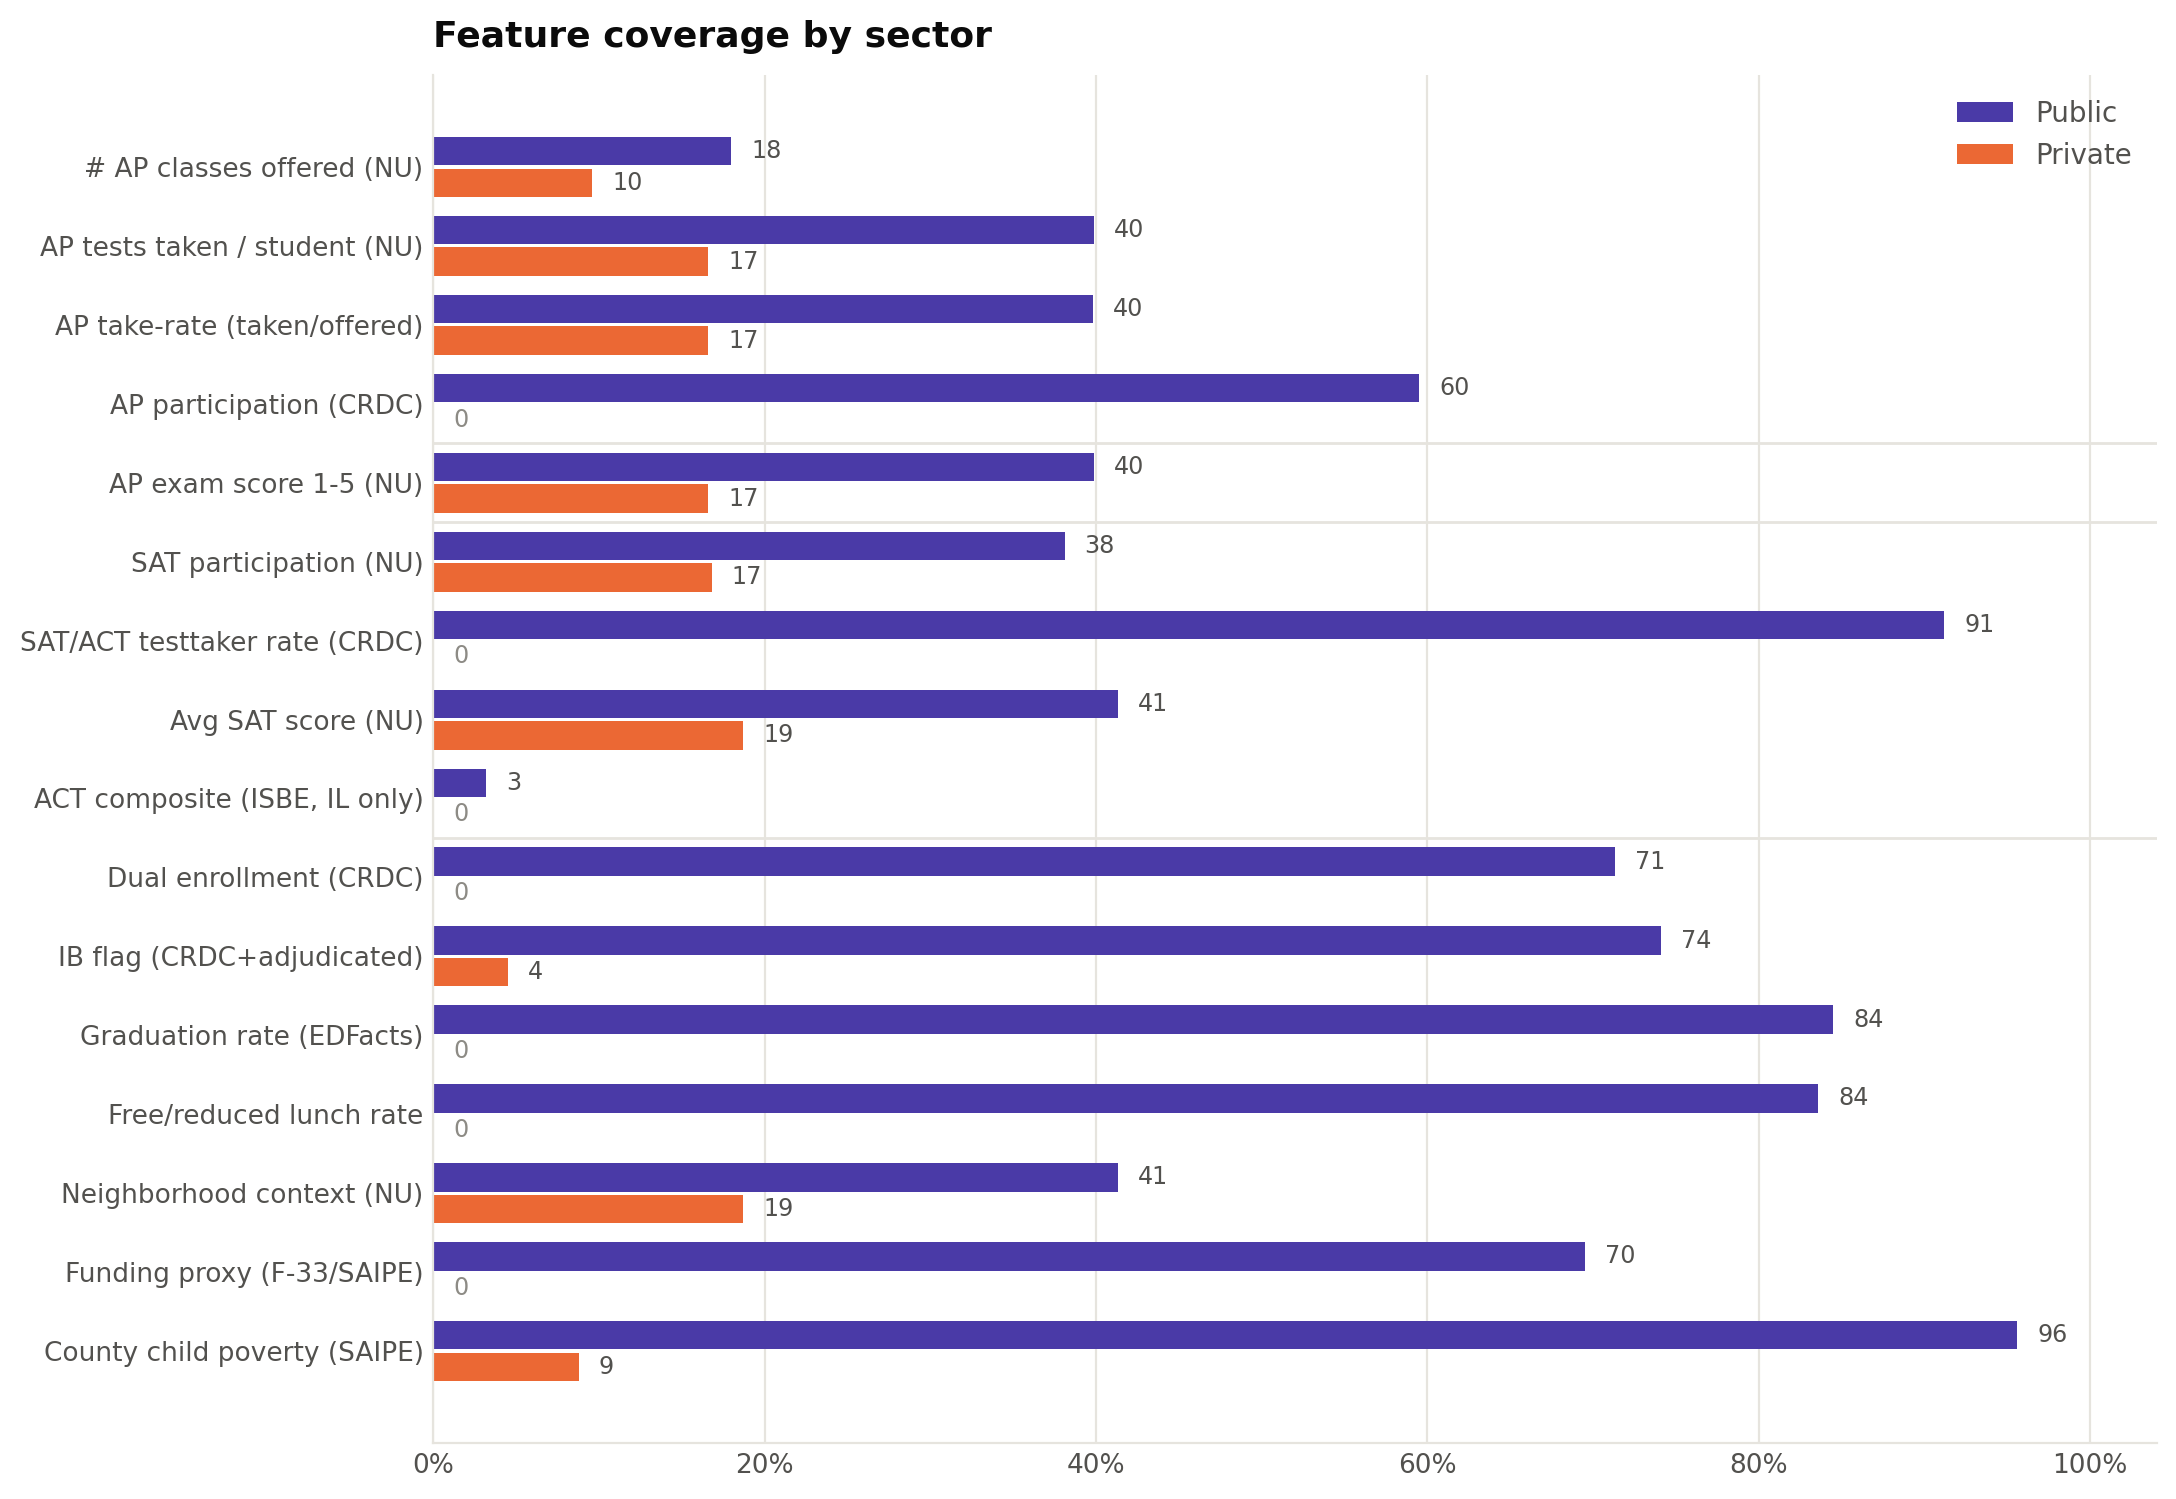
\includegraphics[width=0.86\textwidth]{coverage_by_sector.png}
\caption{Feature-level coverage by sector on the frozen modeling dataset, underneath the component-level view in Figure~\ref{fig:coverage}.}
\label{fig:featcov}
\end{figure}

\begin{figure}[htbp]
\centering
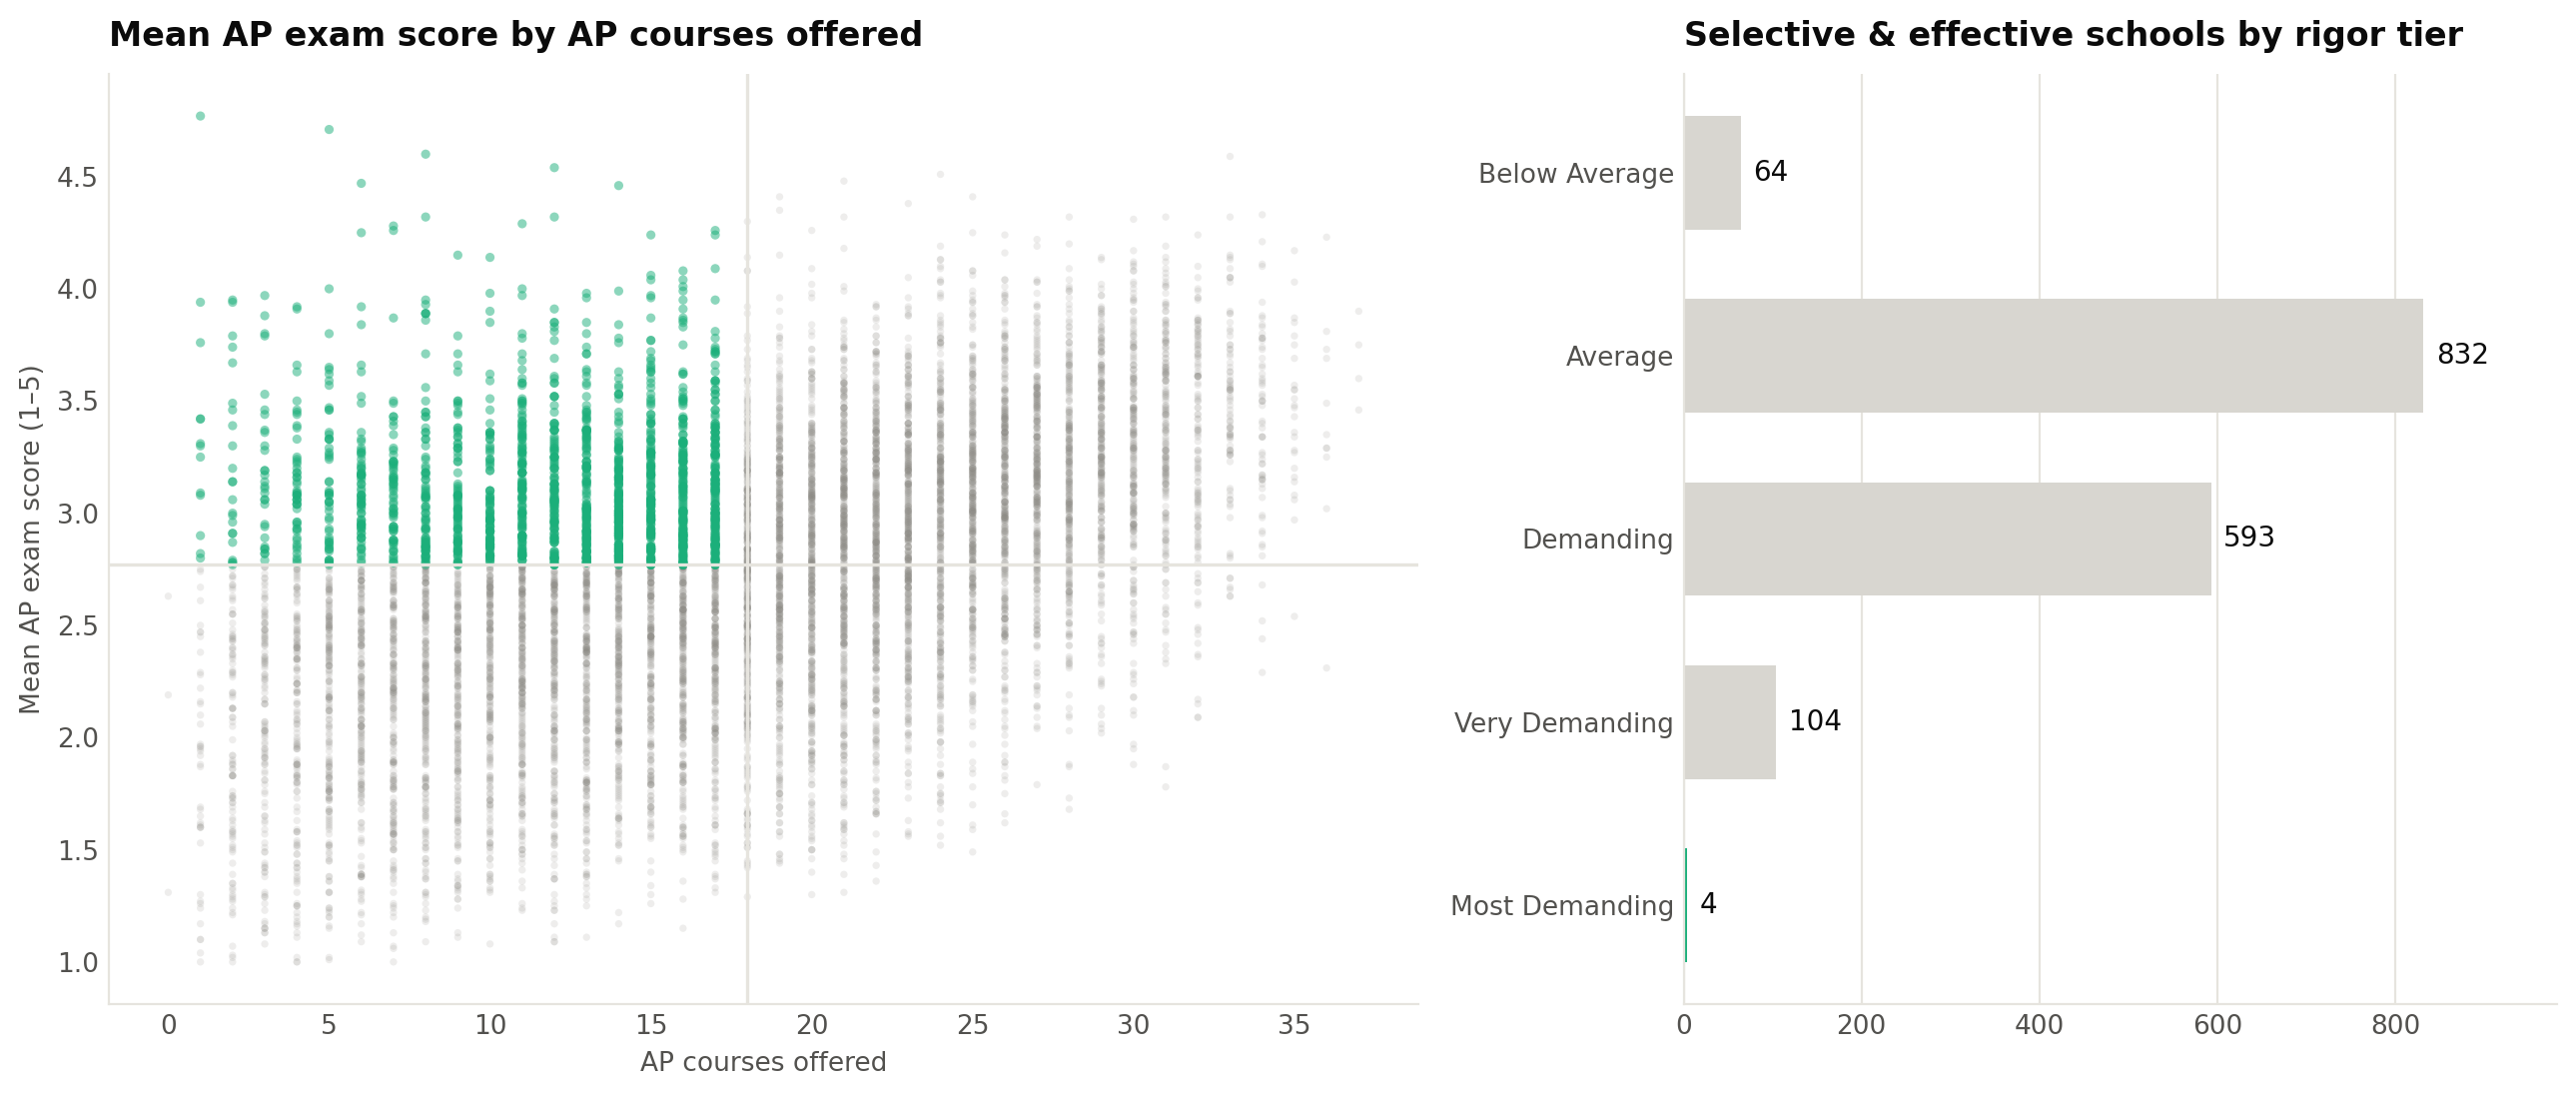
\includegraphics[width=0.78\textwidth]{ap_efficiency.png}
\caption{AP efficiency quadrants. The ``selective and effective'' group --- few offerings, strong exam scores --- is systematically ranked below the top tier by an additive composite.}
\label{fig:apeff}
\end{figure}

\begin{figure}[htbp]
\centering
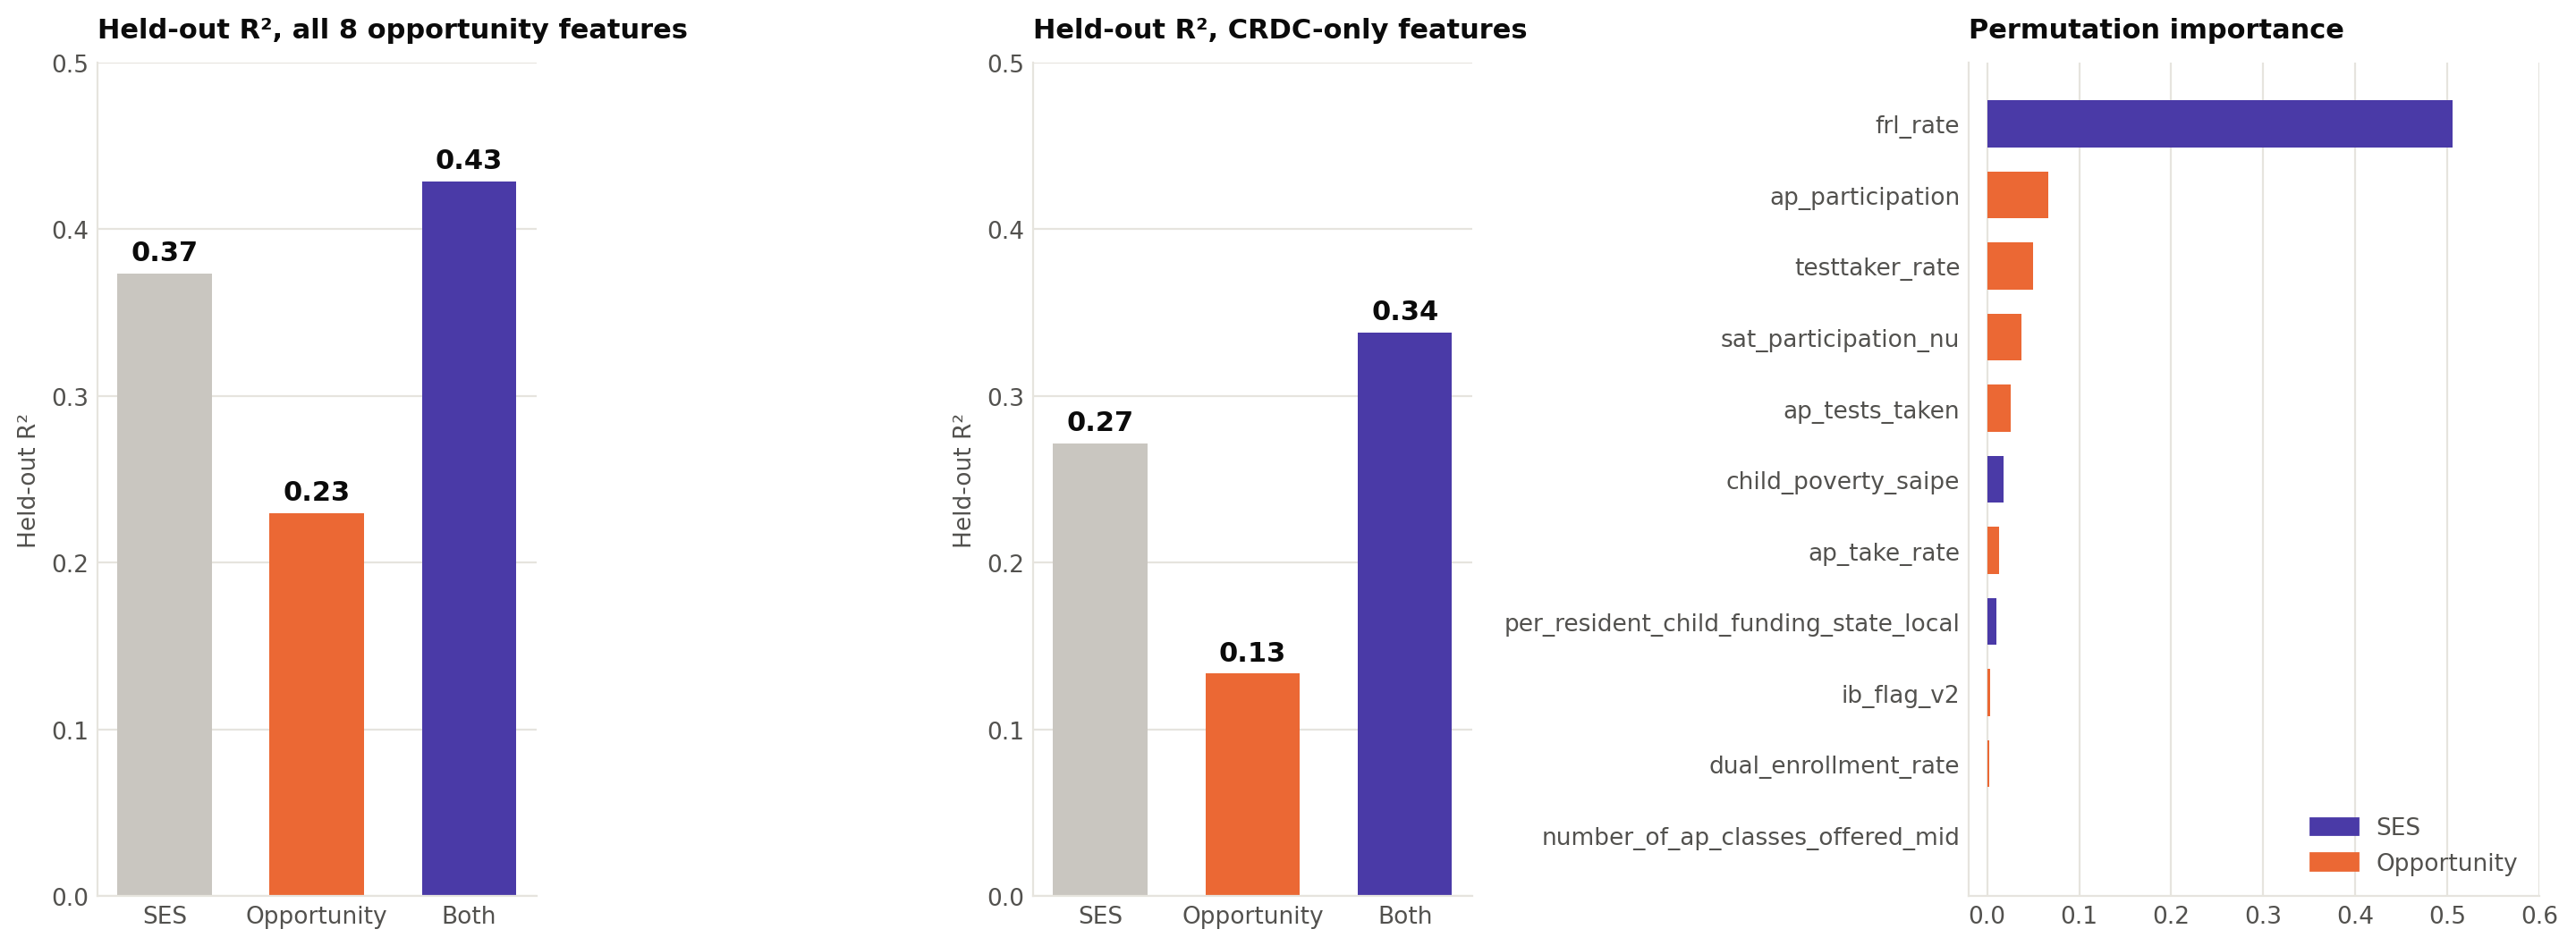
\includegraphics[width=0.84\textwidth]{predictive_validation.png}
\caption{Nested-block predictive validation of the rigor construct's opportunity ingredients against the four-year adjusted cohort graduation rate.}
\label{fig:predictive}
\end{figure}

\clearpage
\section{Cluster Profiles and Index Specification}
\label{app:tables}
\label{app:v5}

\begin{table}[htbp]
\centering
\singlespacing\small
\caption{$k$-means cluster profiles ($k=8$), complete-case subset of 5{,}837 schools. The rigor score is not a clustering input.}
\label{tab:clusters}
\begin{tabular}{@{}rrlrl@{}}
\toprule
Cluster & Size & Character & \% Demanding or above & Top region \\
\midrule
3 & 438   & High funding, high rigor         & 74 & Northeast \\
0 & 724   & High rigor, high test-takers     & 74 & South \\
6 & 25    & High rigor, low AP density       & 92 & West \\
2 & 1{,}029 & High funding, low need          & 44 & Northeast \\
4 & 741   & High AP take-rate, test-takers   & 49 & Midwest \\
7 & 997   & Quiet middle, near average       & 22 & Midwest \\
1 & 1{,}044 & Low funding, low rigor          & 14 & South \\
5 & 839   & High poverty, high need          & 15 & South \\
\bottomrule
\end{tabular}
\end{table}


\begin{center}
\begin{tabular}{@{}lp{6.0cm}rl@{}}
\toprule
Component & Sub-features & Weight & Client factor \\
\midrule
AP opportunity & AP tests taken; tests offered; classes offered (band); take rate; Capstone flag & 0.15 & Advanced curriculum \\
AP performance & AP qualifying density & 0.20 & Advanced curriculum \\
Advanced access & CRDC AP participation; dual-enrollment rate & 0.10 & Advanced curriculum \\
IB & IB intensity & 0.05 & Advanced curriculum \\
STEM depth & CRDC advanced STEM breadth (0--4) & 0.10 & Advanced curriculum \\
Test performance & Mean SAT; ACT composite (Illinois) & 0.20 & Test scores \\
Test participation & Test-taker rate; SAT participation & 0.05 & Test scores \\
College placement & \% to college; \% to four-year (bands) & 0.10 & College placement \\
Faculty investment & \% teachers certified; instructional spend per pupil & 0.05 & Faculty \\
\midrule
\multicolumn{2}{@{}l}{Total} & 1.00 & \\
\bottomrule
\end{tabular}
\end{center}

\medskip
\noindent Two of the client's six stated rigor factors --- extracurricular breadth, and grade point average with academic competitions --- carry no component. No national dataset of high school club offerings exists, and grade point average is neither standardized across schools nor collected federally. These are not deferred items; they cannot be sourced from public data and would have to come from the university's own application records.

\end{document}
